   \documentclass{article}
\usepackage{pgfplots}
\begin{document}
\begin{figure}
\centering

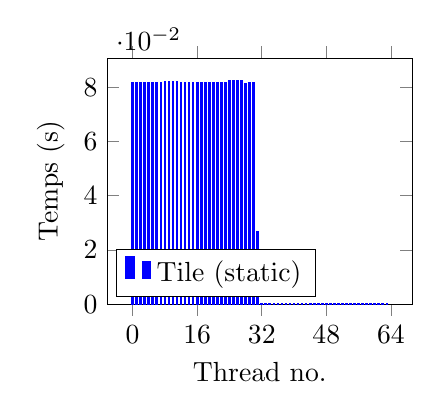
\begin{tikzpicture}
\begin{axis}[
  ybar,
  bar width=0.02cm,
  xlabel={Thread no.},
  ylabel={Temps (s)},
  ymin=0,
  legend pos=south west,
  width=0.45\textwidth,
  xtick distance=16
]

% Données pour le premier graphique (à gauche)
\addplot[color=blue, fill=blue] coordinates {
  (0,0.081537) (1,0.081557) (2,0.081560) (3,0.081565) (4,0.081548) (5,0.081517) (6,0.081567) (7,0.081546) (8,0.081949) (9,0.081946) (10,0.081934) (11,0.081932) (12,0.081512) (13,0.081518) (14,0.081514) (15,0.081526) (16,0.081789) (17,0.081826) (18,0.081796) (19,0.081779) (20,0.081773) (21,0.081762) (22,0.081774) (23,0.081764) (24,0.082400) (25,0.082353) (26,0.082374) (27,0.082427) (28,0.081468) (29,0.081489) (30,0.081496) (31,0.026842) (32,0.000056) (33,0.000055) (34,0.000055) (35,0.000054) (36,0.000055) (37,0.000055) (38,0.000055) (39,0.000055) (40,0.000056) (41,0.000057) (42,0.000056) (43,0.000057) (44,0.000056) (45,0.000056) (46,0.000056) (47,0.000056) (48,0.000054) (49,0.000054) (50,0.000054) (51,0.000054) (52,0.000055) (53,0.000055) (54,0.000056) (55,0.000055) (56,0.000055) (57,0.000057) (58,0.000055) (59,0.000056) (60,0.000056) (61,0.000055) (62,0.000056) (63,0.000054)
};
\addlegendentry{Tile (static)}

\end{axis}
\end{tikzpicture}
\hfill
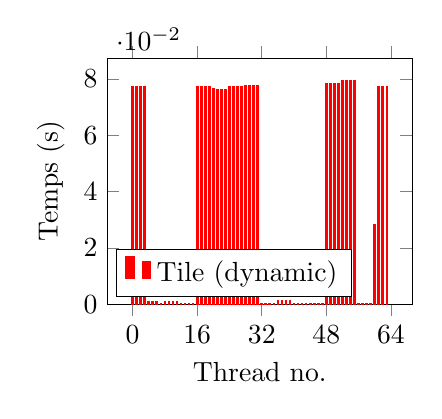
\begin{tikzpicture}
\begin{axis}[
  ybar,
  bar width=0.02cm,
  xlabel={Thread no.},
  ylabel={Temps (s)},
  ymin=0,
  legend pos=south west,
  width=0.45\textwidth,
  xtick distance=16
]

% Données pour le deuxième graphique (au milieu)
\addplot[color=red, fill=red] coordinates {
  (0,0.077432) (1,0.077427) (2,0.077440) (3,0.077437) (4,0.000870) (5,0.000862) (6,0.000867) (7,0.000072) (8,0.001056) (9,0.001046) (10,0.001053) (11,0.001049) (12,0.000070) (13,0.000071) (14,0.000070) (15,0.000071) (16,0.077232) (17,0.077231) (18,0.077216) (19,0.077223) (20,0.076433) (21,0.076248) (22,0.076248) (23,0.076248) (24,0.077380) (25,0.077369) (26,0.077366) (27,0.077370) (28,0.077468) (29,0.077482) (30,0.077468) (31,0.077478) (32,0.000077) (33,0.000077) (34,0.000077) (35,0.000077) (36,0.001364) (37,0.001362) (38,0.001362) (39,0.001366) (40,0.000077) (41,0.000077) (42,0.000077) (43,0.000077) (44,0.000077) (45,0.000077) (46,0.000077) (47,0.000077) (48,0.078229) (49,0.078229) (50,0.078229) (51,0.078230) (52,0.079419) (53,0.079437) (54,0.079420) (55,0.079439) (56,0.000070) (57,0.000070) (58,0.000070) (59,0.000070) (60,0.028246) (61,0.077181) (62,0.077181) (63,0.077181)
};
\addlegendentry{Tile (dynamic)}

\end{axis}
\end{tikzpicture}
\hfill
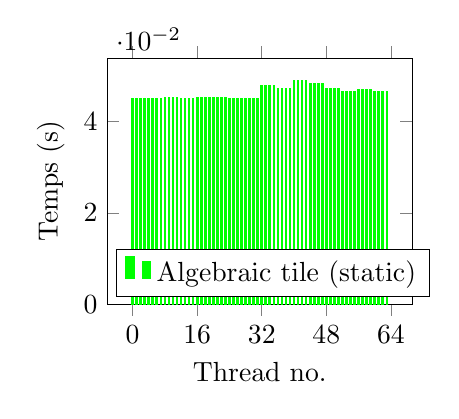
\begin{tikzpicture}
\begin{axis}[
  ybar,
  bar width=0.02cm,
  xlabel={Thread no.},
  ylabel={Temps (s)},
  ymin=0,
  legend pos=south west,
  width=0.45\textwidth,
  xtick distance=16
]

% Données pour le troisième graphique (à droite)
\addplot[color=green, fill=green] coordinates {
  (0,0.045081) (1,0.045052) (2,0.045056) (3,0.045046) (4,0.045118) (5,0.045077) (6,0.045083) (7,0.045078) (8,0.045306) (9,0.045297) (10,0.045288) (11,0.045290) (12,0.045143) (13,0.045138) (14,0.045137) (15,0.045140) (16,0.045313) (17,0.045303) (18,0.045303) (19,0.045308) (20,0.045316) (21,0.045306) (22,0.045307) (23,0.045310) (24,0.045096) (25,0.045076) (26,0.045086) (27,0.045092) (28,0.045092) (29,0.045071) (30,0.045088) (31,0.045084) (32,0.047853) (33,0.047846) (34,0.047847) (35,0.047854) (36,0.047163) (37,0.047159) (38,0.047157) (39,0.047164) (40,0.048988) (41,0.048979) (42,0.048981) (43,0.048978) (44,0.048320) (45,0.048311) (46,0.048312) (47,0.048312) (48,0.047212) (49,0.047199) (50,0.047215) (51,0.047215) (52,0.046645) (53,0.046642) (54,0.046649) (55,0.046624) (56,0.047074) (57,0.047063) (58,0.047067) (59,0.047066) (60,0.046577) (61,0.046546) (62,0.046562) (63,0.046579)
};
\addlegendentry{Algebraic tile (static)}

\end{axis}
\end{tikzpicture}

\caption{Temps d'exécution des threads pour le fichier gemm.c}
\label{fig:graphes}
\end{figure}

\begin{table}[htbp]
  \centering
  \caption{Statistiques pour le fichier gemm.c}
  \begin{tabular}{|c|c|c|c|}
    \hline
    Statistique & Algebraic Tile & Tile (static) & Tile (dynamic) \\ 
    \hline
    Skewness (g1)  & 0.579441 & 0.046933 & 0.0445741 \\ 
    Kurtosis (g2)  & -0.974577 & -1.98542 & -1.98318 \\ 
    Coefficient de variation $ \frac{\sigma}{\overline{x}} $ & 0.0276596 & 1.01278 & 1.00155\\ 
    Percent Imbalance metric en \% & 5.75422 & 105.817 & 107.732\\ 
    Coefficient de Gini  & 0.0150665 & 0.510563 & 0.508482\\ 
    Temps d'exécution (s) &  0.049049    &  0.082575   &  0.079608   \\ 

    \hline
  \end{tabular}
\end{table}
g1=$ \frac{\sum_{i=1}^{n} (x_i - \overline{x})^3}{n\sigma^3} $\
g2=$ \frac{\sum_{i=1}^{n} (x_i - \overline{x})^4}{n\sigma^4} $\
Coefficient de Gini = $ \frac{\sum_{i=1}^{n}\sum_{j=1}^{n} |x_i - x_j|}{2n^2\overline{x}} $\
\newpage

\begin{figure}
\centering

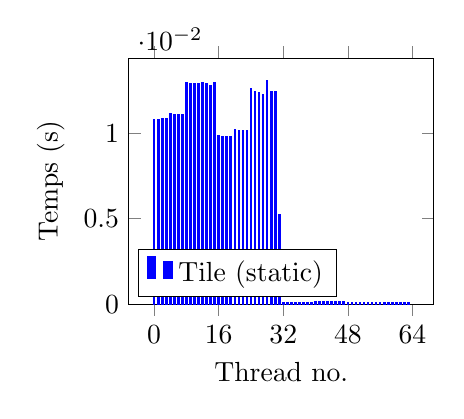
\begin{tikzpicture}
\begin{axis}[
  ybar,
  bar width=0.02cm,
  xlabel={Thread no.},
  ylabel={Temps (s)},
  ymin=0,
  legend pos=south west,
  width=0.45\textwidth,
  xtick distance=16
]

% Données pour le premier graphique (à gauche)
\addplot[color=blue, fill=blue] coordinates {
  (0,0.010788) (1,0.010798) (2,0.010833) (3,0.010848) (4,0.011138) (5,0.011092) (6,0.011093) (7,0.011085) (8,0.012975) (9,0.012891) (10,0.012885) (11,0.012884) (12,0.012969) (13,0.012926) (14,0.012783) (15,0.012927) (16,0.009842) (17,0.009794) (18,0.009775) (19,0.009783) (20,0.010237) (21,0.010173) (22,0.010155) (23,0.010167) (24,0.012596) (25,0.012422) (26,0.012344) (27,0.012256) (28,0.013076) (29,0.012402) (30,0.012412) (31,0.005222) (32,0.000119) (33,0.000119) (34,0.000119) (35,0.000119) (36,0.000122) (37,0.000122) (38,0.000122) (39,0.000122) (40,0.000126) (41,0.000126) (42,0.000126) (43,0.000126) (44,0.000125) (45,0.000125) (46,0.000125) (47,0.000125) (48,0.000121) (49,0.000120) (50,0.000120) (51,0.000121) (52,0.000122) (53,0.000123) (54,0.000122) (55,0.000123) (56,0.000122) (57,0.000122) (58,0.000121) (59,0.000122) (60,0.000120) (61,0.000121) (62,0.000120) (63,0.000121)
};
\addlegendentry{Tile (static)}

\end{axis}
\end{tikzpicture}
\hfill
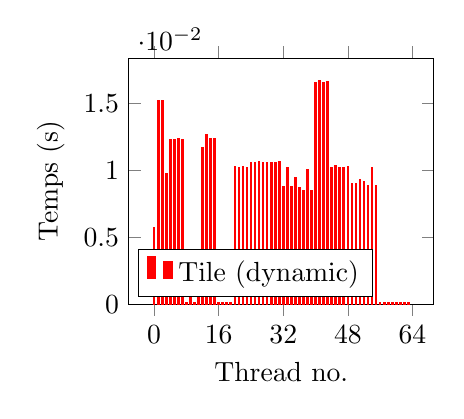
\begin{tikzpicture}
\begin{axis}[
  ybar,
  bar width=0.02cm,
  xlabel={Thread no.},
  ylabel={Temps (s)},
  ymin=0,
  legend pos=south west,
  width=0.45\textwidth,
  xtick distance=16
]

% Données pour le deuxième graphique (au milieu)
\addplot[color=red, fill=red] coordinates {
  (0,0.005712) (1,0.015205) (2,0.015258) (3,0.009749) (4,0.012309) (5,0.012343) (6,0.012411) (7,0.012333) (8,0.000120) (9,0.002804) (10,0.000121) (11,0.003513) (12,0.011714) (13,0.012656) (14,0.012378) (15,0.012397) (16,0.000122) (17,0.000122) (18,0.000122) (19,0.000122) (20,0.010269) (21,0.010232) (22,0.010300) (23,0.010231) (24,0.010577) (25,0.010569) (26,0.010650) (27,0.010580) (28,0.010618) (29,0.010591) (30,0.010615) (31,0.010667) (32,0.008788) (33,0.010248) (34,0.008788) (35,0.009499) (36,0.008751) (37,0.008532) (38,0.010051) (39,0.008532) (40,0.016599) (41,0.016732) (42,0.016562) (43,0.016645) (44,0.010238) (45,0.010348) (46,0.010241) (47,0.010208) (48,0.010260) (49,0.009048) (50,0.009047) (51,0.009310) (52,0.009198) (53,0.008853) (54,0.010224) (55,0.008850) (56,0.000125) (57,0.000125) (58,0.000125) (59,0.000125) (60,0.000127) (61,0.000127) (62,0.000127) (63,0.000126)
};
\addlegendentry{Tile (dynamic)}

\end{axis}
\end{tikzpicture}
\hfill
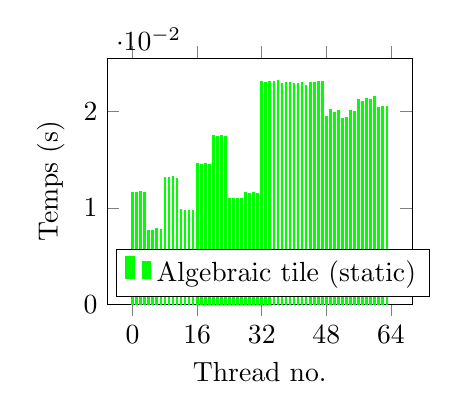
\begin{tikzpicture}
\begin{axis}[
  ybar,
  bar width=0.02cm,
  xlabel={Thread no.},
  ylabel={Temps (s)},
  ymin=0,
  legend pos=south west,
  width=0.45\textwidth,
  xtick distance=16
]

% Données pour le troisième graphique (à droite)
\addplot[color=green, fill=green] coordinates {
  (0,0.011597) (1,0.011544) (2,0.011643) (3,0.011559) (4,0.007593) (5,0.007695) (6,0.007801) (7,0.007704) (8,0.013177) (9,0.013120) (10,0.013219) (11,0.013074) (12,0.009789) (13,0.009748) (14,0.009738) (15,0.009725) (16,0.014586) (17,0.014499) (18,0.014560) (19,0.014546) (20,0.017509) (21,0.017414) (22,0.017502) (23,0.017411) (24,0.010980) (25,0.010922) (26,0.011001) (27,0.010953) (28,0.011565) (29,0.011489) (30,0.011554) (31,0.011515) (32,0.023128) (33,0.023048) (34,0.023074) (35,0.023078) (36,0.023225) (37,0.022949) (38,0.023035) (39,0.023003) (40,0.022931) (41,0.022872) (42,0.023055) (43,0.022722) (44,0.023009) (45,0.022966) (46,0.023087) (47,0.023159) (48,0.019463) (49,0.020214) (50,0.019946) (51,0.020137) (52,0.019266) (53,0.019419) (54,0.020152) (55,0.020011) (56,0.021292) (57,0.021053) (58,0.021319) (59,0.021208) (60,0.021525) (61,0.020404) (62,0.020505) (63,0.020511)
};
\addlegendentry{Algebraic tile (static)}

\end{axis}
\end{tikzpicture}

\caption{Temps d'exécution des threads pour le fichier gemver.c}
\label{fig:graphes}
\end{figure}

\begin{table}[htbp]
  \centering
  \caption{Statistiques pour le fichier gemver.c}
  \begin{tabular}{|c|c|c|c|}
    \hline
    Statistique & Algebraic Tile & Tile (static) & Tile (dynamic) \\ 
    \hline
    Skewness (g1)  & -0.257408 & 0.0985219 & -0.559069 \\ 
    Kurtosis (g2)  & -1.47141 & -1.89693 & -0.70361 \\ 
    Coefficient de variation $ \frac{\sigma}{\overline{x}} $ & 0.313463 & 0.998647 & 0.598304\\ 
    Percent Imbalance metric en \% & 37.439 & 127.731 & 100.545\\ 
    Coefficient de Gini  & 0.176691 & 0.525185 & 0.31933\\ 
    Temps d'exécution (s) &  0.023461    &  0.013363   &  0.020933   \\ 

    \hline
  \end{tabular}
\end{table}
g1=$ \frac{\sum_{i=1}^{n} (x_i - \overline{x})^3}{n\sigma^3} $\
g2=$ \frac{\sum_{i=1}^{n} (x_i - \overline{x})^4}{n\sigma^4} $\
Coefficient de Gini = $ \frac{\sum_{i=1}^{n}\sum_{j=1}^{n} |x_i - x_j|}{2n^2\overline{x}} $\
\newpage

\begin{figure}
\centering

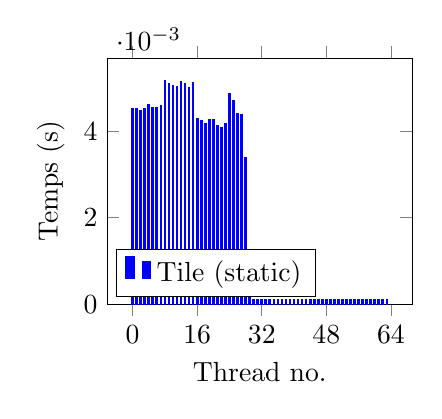
\begin{tikzpicture}
\begin{axis}[
  ybar,
  bar width=0.02cm,
  xlabel={Thread no.},
  ylabel={Temps (s)},
  ymin=0,
  legend pos=south west,
  width=0.45\textwidth,
  xtick distance=16
]

% Données pour le premier graphique (à gauche)
\addplot[color=blue, fill=blue] coordinates {
  (0,0.004512) (1,0.004510) (2,0.004486) (3,0.004531) (4,0.004606) (5,0.004554) (6,0.004539) (7,0.004582) (8,0.005170) (9,0.005105) (10,0.005060) (11,0.005034) (12,0.005140) (13,0.005107) (14,0.005010) (15,0.005132) (16,0.004299) (17,0.004245) (18,0.004177) (19,0.004263) (20,0.004262) (21,0.004119) (22,0.004093) (23,0.004184) (24,0.004875) (25,0.004696) (26,0.004400) (27,0.004382) (28,0.003379) (29,0.000447) (30,0.000101) (31,0.000102) (32,0.000107) (33,0.000108) (34,0.000107) (35,0.000107) (36,0.000109) (37,0.000108) (38,0.000108) (39,0.000108) (40,0.000110) (41,0.000110) (42,0.000110) (43,0.000110) (44,0.000110) (45,0.000110) (46,0.000110) (47,0.000110) (48,0.000104) (49,0.000104) (50,0.000104) (51,0.000105) (52,0.000106) (53,0.000106) (54,0.000106) (55,0.000106) (56,0.000106) (57,0.000106) (58,0.000106) (59,0.000106) (60,0.000105) (61,0.000105) (62,0.000105) (63,0.000105)
};
\addlegendentry{Tile (static)}

\end{axis}
\end{tikzpicture}
\hfill
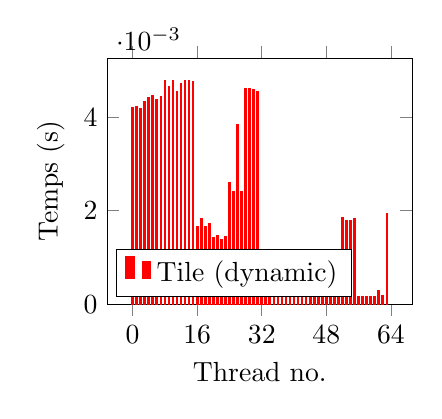
\begin{tikzpicture}
\begin{axis}[
  ybar,
  bar width=0.02cm,
  xlabel={Thread no.},
  ylabel={Temps (s)},
  ymin=0,
  legend pos=south west,
  width=0.45\textwidth,
  xtick distance=16
]

% Données pour le deuxième graphique (au milieu)
\addplot[color=red, fill=red] coordinates {
  (0,0.004208) (1,0.004236) (2,0.004190) (3,0.004339) (4,0.004417) (5,0.004456) (6,0.004373) (7,0.004450) (8,0.004778) (9,0.004661) (10,0.004778) (11,0.004545) (12,0.004718) (13,0.004783) (14,0.004772) (15,0.004769) (16,0.001665) (17,0.001834) (18,0.001669) (19,0.001714) (20,0.001415) (21,0.001475) (22,0.001376) (23,0.001455) (24,0.002593) (25,0.002399) (26,0.003834) (27,0.002402) (28,0.004604) (29,0.004621) (30,0.004593) (31,0.004546) (32,0.000173) (33,0.000173) (34,0.000173) (35,0.000173) (36,0.000166) (37,0.000170) (38,0.000170) (39,0.000170) (40,0.000170) (41,0.000170) (42,0.000170) (43,0.000170) (44,0.000174) (45,0.000171) (46,0.000171) (47,0.000171) (48,0.000182) (49,0.000182) (50,0.000176) (51,0.000176) (52,0.001843) (53,0.001797) (54,0.001789) (55,0.001825) (56,0.000170) (57,0.000169) (58,0.000170) (59,0.000170) (60,0.000169) (61,0.000288) (62,0.000175) (63,0.001935)
};
\addlegendentry{Tile (dynamic)}

\end{axis}
\end{tikzpicture}
\hfill
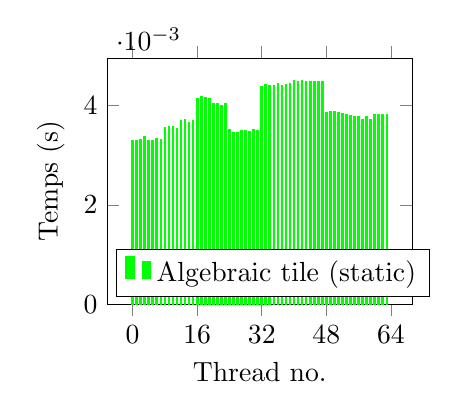
\begin{tikzpicture}
\begin{axis}[
  ybar,
  bar width=0.02cm,
  xlabel={Thread no.},
  ylabel={Temps (s)},
  ymin=0,
  legend pos=south west,
  width=0.45\textwidth,
  xtick distance=16
]

% Données pour le troisième graphique (à droite)
\addplot[color=green, fill=green] coordinates {
  (0,0.003299) (1,0.003291) (2,0.003320) (3,0.003366) (4,0.003302) (5,0.003294) (6,0.003339) (7,0.003310) (8,0.003556) (9,0.003576) (10,0.003585) (11,0.003541) (12,0.003697) (13,0.003708) (14,0.003664) (15,0.003696) (16,0.004145) (17,0.004175) (18,0.004168) (19,0.004147) (20,0.004039) (21,0.004041) (22,0.004004) (23,0.004037) (24,0.003516) (25,0.003450) (26,0.003455) (27,0.003498) (28,0.003504) (29,0.003483) (30,0.003516) (31,0.003486) (32,0.004389) (33,0.004417) (34,0.004401) (35,0.004395) (36,0.004434) (37,0.004406) (38,0.004413) (39,0.004433) (40,0.004504) (41,0.004483) (42,0.004498) (43,0.004476) (44,0.004480) (45,0.004480) (46,0.004487) (47,0.004479) (48,0.003867) (49,0.003872) (50,0.003870) (51,0.003863) (52,0.003832) (53,0.003809) (54,0.003801) (55,0.003777) (56,0.003769) (57,0.003711) (58,0.003779) (59,0.003710) (60,0.003817) (61,0.003819) (62,0.003821) (63,0.003816)
};
\addlegendentry{Algebraic tile (static)}

\end{axis}
\end{tikzpicture}

\caption{Temps d'exécution des threads pour le fichier gesummv.c}
\label{fig:graphes}
\end{figure}

\begin{table}[htbp]
  \centering
  \caption{Statistiques pour le fichier gesummv.c}
  \begin{tabular}{|c|c|c|c|}
    \hline
    Statistique & Algebraic Tile & Tile (static) & Tile (dynamic) \\ 
    \hline
    Skewness (g1)  & 0.246103 & 0.23231 & 0.40013 \\ 
    Kurtosis (g2)  & -1.21971 & -1.88883 & -1.53112 \\ 
    Coefficient de variation $ \frac{\sigma}{\overline{x}} $ & 0.102127 & 1.04691 & 0.934228\\ 
    Percent Imbalance metric en \% & 16.0843 & 142.351 & 137.999\\ 
    Coefficient de Gini  & 0.0580957 & 0.540321 & 0.50786\\ 
    Temps d'exécution (s) &  0.004573    &  0.005239   &  0.004905   \\ 

    \hline
  \end{tabular}
\end{table}
g1=$ \frac{\sum_{i=1}^{n} (x_i - \overline{x})^3}{n\sigma^3} $\
g2=$ \frac{\sum_{i=1}^{n} (x_i - \overline{x})^4}{n\sigma^4} $\
Coefficient de Gini = $ \frac{\sum_{i=1}^{n}\sum_{j=1}^{n} |x_i - x_j|}{2n^2\overline{x}} $\
\newpage

\begin{figure}
\centering

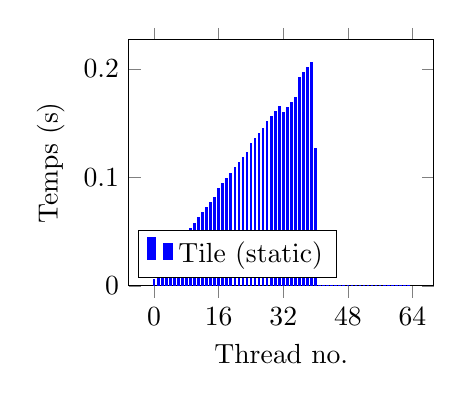
\begin{tikzpicture}
\begin{axis}[
  ybar,
  bar width=0.02cm,
  xlabel={Thread no.},
  ylabel={Temps (s)},
  ymin=0,
  legend pos=south west,
  width=0.45\textwidth,
  xtick distance=16
]

% Données pour le premier graphique (à gauche)
\addplot[color=blue, fill=blue] coordinates {
  (0,0.005327) (1,0.011674) (2,0.016573) (3,0.021800) (4,0.026722) (5,0.031848) (6,0.036913) (7,0.041916) (8,0.047995) (9,0.052944) (10,0.057835) (11,0.062705) (12,0.067525) (13,0.072289) (14,0.076978) (15,0.081681) (16,0.089243) (17,0.093968) (18,0.098696) (19,0.103260) (20,0.108841) (21,0.113494) (22,0.118104) (23,0.122797) (24,0.131255) (25,0.135890) (26,0.140617) (27,0.145201) (28,0.151578) (29,0.156383) (30,0.160907) (31,0.165533) (32,0.159457) (33,0.164050) (34,0.168960) (35,0.173588) (36,0.192315) (37,0.196928) (38,0.201648) (39,0.206314) (40,0.126209) (41,0.000051) (42,0.000051) (43,0.000051) (44,0.000051) (45,0.000051) (46,0.000051) (47,0.000051) (48,0.000048) (49,0.000048) (50,0.000048) (51,0.000048) (52,0.000048) (53,0.000048) (54,0.000048) (55,0.000048) (56,0.000048) (57,0.000048) (58,0.000048) (59,0.000048) (60,0.000049) (61,0.000049) (62,0.000049) (63,0.000049)
};
\addlegendentry{Tile (static)}

\end{axis}
\end{tikzpicture}
\hfill
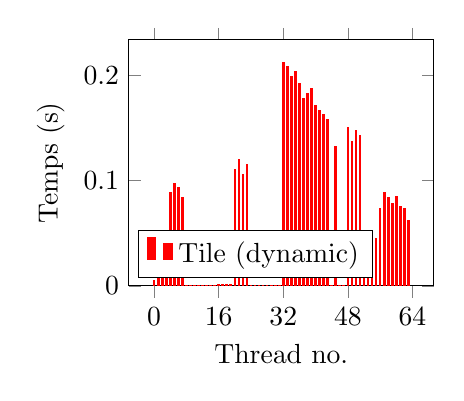
\begin{tikzpicture}
\begin{axis}[
  ybar,
  bar width=0.02cm,
  xlabel={Thread no.},
  ylabel={Temps (s)},
  ymin=0,
  legend pos=south west,
  width=0.45\textwidth,
  xtick distance=16
]

% Données pour le deuxième graphique (au milieu)
\addplot[color=red, fill=red] coordinates {
  (0,0.004982) (1,0.022294) (2,0.016106) (3,0.010914) (4,0.088314) (5,0.097717) (6,0.093102) (7,0.083711) (8,0.000063) (9,0.000064) (10,0.000065) (11,0.000064) (12,0.000227) (13,0.000254) (14,0.000243) (15,0.000216) (16,0.000858) (17,0.000863) (18,0.000816) (19,0.000834) (20,0.111014) (21,0.120397) (22,0.106065) (23,0.115763) (24,0.000444) (25,0.000445) (26,0.000430) (27,0.000416) (28,0.000064) (29,0.000064) (30,0.000064) (31,0.000064) (32,0.212892) (33,0.208235) (34,0.198875) (35,0.203556) (36,0.192278) (37,0.178196) (38,0.182886) (39,0.187629) (40,0.171875) (41,0.166867) (42,0.162606) (43,0.157823) (44,0.000088) (45,0.132579) (46,0.000660) (47,0.000675) (48,0.150961) (49,0.137664) (50,0.147581) (51,0.142786) (52,0.035130) (53,0.029874) (54,0.040503) (55,0.045390) (56,0.073782) (57,0.089019) (58,0.084250) (59,0.078696) (60,0.084584) (61,0.075590) (62,0.073378) (63,0.062257)
};
\addlegendentry{Tile (dynamic)}

\end{axis}
\end{tikzpicture}
\hfill
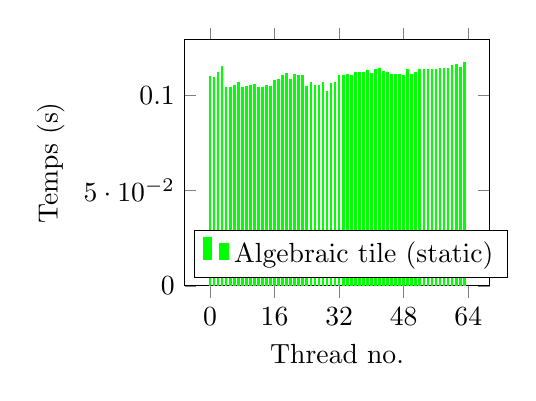
\begin{tikzpicture}
\begin{axis}[
  ybar,
  bar width=0.02cm,
  xlabel={Thread no.},
  ylabel={Temps (s)},
  ymin=0,
  legend pos=south west,
  width=0.45\textwidth,
  xtick distance=16
]

% Données pour le troisième graphique (à droite)
\addplot[color=green, fill=green] coordinates {
  (0,0.109906) (1,0.109337) (2,0.112085) (3,0.115152) (4,0.104364) (5,0.104396) (6,0.105175) (7,0.106894) (8,0.104325) (9,0.104582) (10,0.105218) (11,0.106040) (12,0.104235) (13,0.104086) (14,0.105169) (15,0.105045) (16,0.108150) (17,0.108665) (18,0.110543) (19,0.111742) (20,0.108379) (21,0.110901) (22,0.110698) (23,0.110637) (24,0.104629) (25,0.106746) (26,0.105424) (27,0.105493) (28,0.106984) (29,0.102350) (30,0.106476) (31,0.106943) (32,0.110584) (33,0.110686) (34,0.111294) (35,0.110538) (36,0.112047) (37,0.112083) (38,0.112295) (39,0.112987) (40,0.111459) (41,0.113860) (42,0.114430) (43,0.112442) (44,0.112112) (45,0.110914) (46,0.110950) (47,0.111012) (48,0.110707) (49,0.113832) (50,0.110967) (51,0.112222) (52,0.113603) (53,0.113625) (54,0.113665) (55,0.113851) (56,0.113981) (57,0.114037) (58,0.114111) (59,0.114277) (60,0.115790) (61,0.116135) (62,0.114789) (63,0.117646)
};
\addlegendentry{Algebraic tile (static)}

\end{axis}
\end{tikzpicture}

\caption{Temps d'exécution des threads pour le fichier syr2k.c}
\label{fig:graphes}
\end{figure}

\begin{table}[htbp]
  \centering
  \caption{Statistiques pour le fichier syr2k.c}
  \begin{tabular}{|c|c|c|c|}
    \hline
    Statistique & Algebraic Tile & Tile (static) & Tile (dynamic) \\ 
    \hline
    Skewness (g1)  & -0.245009 & 0.497711 & 0.49733 \\ 
    Kurtosis (g2)  & -1.03816 & -1.20161 & -1.17107 \\ 
    Coefficient de variation $ \frac{\sigma}{\overline{x}} $ & 0.0340169 & 1.0107 & 1.00003\\ 
    Percent Imbalance metric en \% & 6.89455 & 204.306 & 197.095\\ 
    Coefficient de Gini  & 0.0193106 & 0.559804 & 0.554393\\ 
    Temps d'exécution (s) &  0.118044    &  0.206434   &  0.214200   \\ 

    \hline
  \end{tabular}
\end{table}
g1=$ \frac{\sum_{i=1}^{n} (x_i - \overline{x})^3}{n\sigma^3} $\
g2=$ \frac{\sum_{i=1}^{n} (x_i - \overline{x})^4}{n\sigma^4} $\
Coefficient de Gini = $ \frac{\sum_{i=1}^{n}\sum_{j=1}^{n} |x_i - x_j|}{2n^2\overline{x}} $\
\newpage

\begin{figure}
\centering

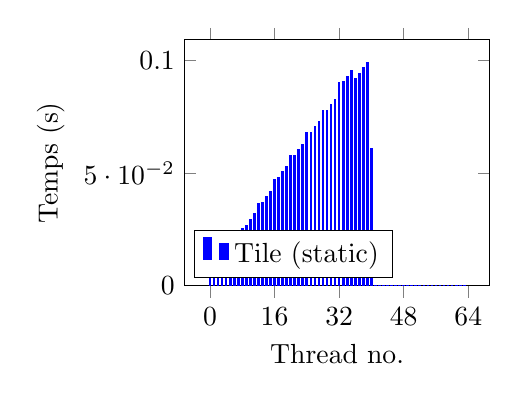
\begin{tikzpicture}
\begin{axis}[
  ybar,
  bar width=0.02cm,
  xlabel={Thread no.},
  ylabel={Temps (s)},
  ymin=0,
  legend pos=south west,
  width=0.45\textwidth,
  xtick distance=16
]

% Données pour le premier graphique (à gauche)
\addplot[color=blue, fill=blue] coordinates {
  (0,0.003089) (1,0.004591) (2,0.007148) (3,0.009872) (4,0.013410) (5,0.015534) (6,0.018246) (7,0.020945) (8,0.025465) (9,0.026781) (10,0.029424) (11,0.032028) (12,0.036436) (13,0.037032) (14,0.039540) (15,0.042014) (16,0.047104) (17,0.048048) (18,0.050494) (19,0.052929) (20,0.057785) (21,0.057904) (22,0.060346) (23,0.062759) (24,0.067767) (25,0.068080) (26,0.070541) (27,0.072971) (28,0.077800) (29,0.077948) (30,0.080339) (31,0.082804) (32,0.090287) (33,0.090582) (34,0.093024) (35,0.095491) (36,0.091974) (37,0.094267) (38,0.096729) (39,0.099217) (40,0.061008) (41,0.000054) (42,0.000053) (43,0.000053) (44,0.000053) (45,0.000054) (46,0.000053) (47,0.000053) (48,0.000051) (49,0.000050) (50,0.000051) (51,0.000050) (52,0.000050) (53,0.000050) (54,0.000050) (55,0.000050) (56,0.000051) (57,0.000051) (58,0.000051) (59,0.000051) (60,0.000054) (61,0.000054) (62,0.000054) (63,0.000054)
};
\addlegendentry{Tile (static)}

\end{axis}
\end{tikzpicture}
\hfill
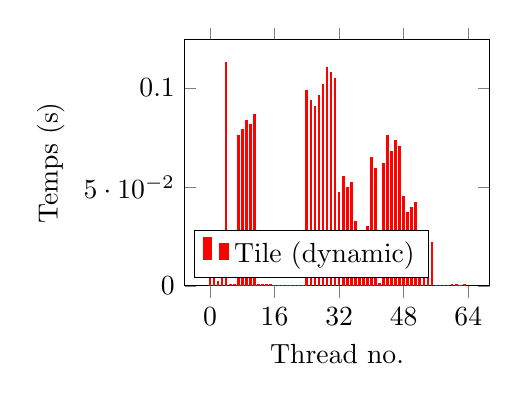
\begin{tikzpicture}
\begin{axis}[
  ybar,
  bar width=0.02cm,
  xlabel={Thread no.},
  ylabel={Temps (s)},
  ymin=0,
  legend pos=south west,
  width=0.45\textwidth,
  xtick distance=16
]

% Données pour le deuxième graphique (au milieu)
\addplot[color=red, fill=red] coordinates {
  (0,0.005517) (1,0.010535) (2,0.002378) (3,0.008109) (4,0.112988) (5,0.000503) (6,0.000516) (7,0.076087) (8,0.078854) (9,0.083637) (10,0.081541) (11,0.086354) (12,0.000659) (13,0.000682) (14,0.000614) (15,0.000639) (16,0.000063) (17,0.000063) (18,0.000063) (19,0.000063) (20,0.000062) (21,0.000062) (22,0.000062) (23,0.000062) (24,0.098832) (25,0.093432) (26,0.090666) (27,0.096127) (28,0.101834) (29,0.110145) (30,0.107541) (31,0.104688) (32,0.046891) (33,0.054943) (34,0.049570) (35,0.052263) (36,0.032363) (37,0.024323) (38,0.027007) (39,0.029691) (40,0.064829) (41,0.059392) (42,0.001220) (43,0.061842) (44,0.075973) (45,0.067712) (46,0.073253) (47,0.070468) (48,0.045019) (49,0.036907) (50,0.039583) (51,0.042267) (52,0.019028) (53,0.016203) (54,0.013527) (55,0.021705) (56,0.000067) (57,0.000067) (58,0.000067) (59,0.000342) (60,0.000495) (61,0.000489) (62,0.000324) (63,0.000467)
};
\addlegendentry{Tile (dynamic)}

\end{axis}
\end{tikzpicture}
\hfill
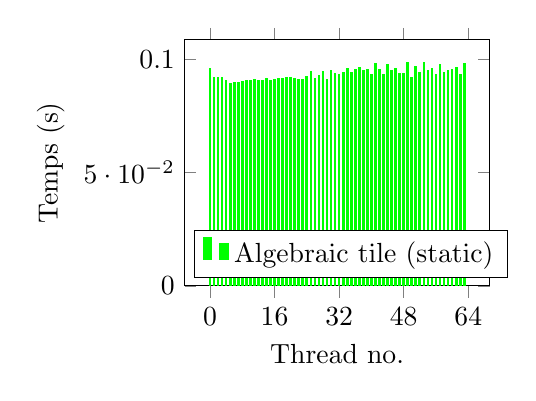
\begin{tikzpicture}
\begin{axis}[
  ybar,
  bar width=0.02cm,
  xlabel={Thread no.},
  ylabel={Temps (s)},
  ymin=0,
  legend pos=south west,
  width=0.45\textwidth,
  xtick distance=16
]

% Données pour le troisième graphique (à droite)
\addplot[color=green, fill=green] coordinates {
  (0,0.096128) (1,0.092136) (2,0.092070) (3,0.092148) (4,0.090599) (5,0.089438) (6,0.089836) (7,0.089656) (8,0.090381) (9,0.090664) (10,0.090834) (11,0.091139) (12,0.090543) (13,0.090429) (14,0.091390) (15,0.090511) (16,0.091128) (17,0.091732) (18,0.091737) (19,0.092113) (20,0.091795) (21,0.091682) (22,0.091224) (23,0.091157) (24,0.092612) (25,0.094779) (26,0.091653) (27,0.093044) (28,0.094522) (29,0.091145) (30,0.095081) (31,0.093896) (32,0.093283) (33,0.094299) (34,0.095724) (35,0.094233) (36,0.095326) (37,0.096206) (38,0.094950) (39,0.095520) (40,0.093470) (41,0.098203) (42,0.095562) (43,0.093481) (44,0.097610) (45,0.095010) (46,0.096064) (47,0.093723) (48,0.093703) (49,0.098462) (50,0.092080) (51,0.096781) (52,0.094134) (53,0.098771) (54,0.095093) (55,0.095935) (56,0.093136) (57,0.097785) (58,0.094160) (59,0.095163) (60,0.095376) (61,0.096350) (62,0.093337) (63,0.098115)
};
\addlegendentry{Algebraic tile (static)}

\end{axis}
\end{tikzpicture}

\caption{Temps d'exécution des threads pour le fichier syrk.c}
\label{fig:graphes}
\end{figure}

\begin{table}[htbp]
  \centering
  \caption{Statistiques pour le fichier syrk.c}
  \begin{tabular}{|c|c|c|c|}
    \hline
    Statistique & Algebraic Tile & Tile (static) & Tile (dynamic) \\ 
    \hline
    Skewness (g1)  & 0.293362 & 0.469831 & 0.534365 \\ 
    Kurtosis (g2)  & -0.852805 & -1.28275 & -1.1806 \\ 
    Coefficient de variation $ \frac{\sigma}{\overline{x}} $ & 0.0259525 & 1.00921 & 1.02085\\ 
    Percent Imbalance metric en \% & 5.56247 & 187.202 & 203.619\\ 
    Coefficient de Gini  & 0.0148267 & 0.558979 & 0.564035\\ 
    Temps d'exécution (s) &  0.099025    &  0.099317   &  0.113853   \\ 

    \hline
  \end{tabular}
\end{table}
g1=$ \frac{\sum_{i=1}^{n} (x_i - \overline{x})^3}{n\sigma^3} $\
g2=$ \frac{\sum_{i=1}^{n} (x_i - \overline{x})^4}{n\sigma^4} $\
Coefficient de Gini = $ \frac{\sum_{i=1}^{n}\sum_{j=1}^{n} |x_i - x_j|}{2n^2\overline{x}} $\
\newpage

\begin{figure}
\centering

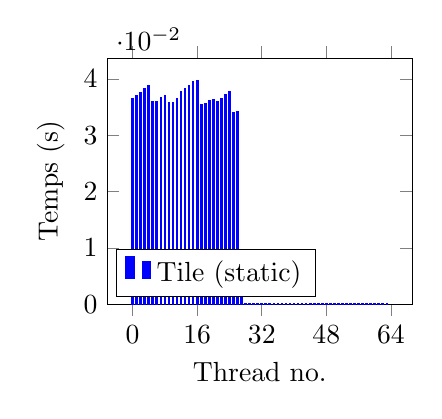
\begin{tikzpicture}
\begin{axis}[
  ybar,
  bar width=0.02cm,
  xlabel={Thread no.},
  ylabel={Temps (s)},
  ymin=0,
  legend pos=south west,
  width=0.45\textwidth,
  xtick distance=16
]

% Données pour le premier graphique (à gauche)
\addplot[color=blue, fill=blue] coordinates {
  (0,0.036605) (1,0.037014) (2,0.037516) (3,0.038326) (4,0.038857) (5,0.035965) (6,0.036056) (7,0.036643) (8,0.036974) (9,0.035726) (10,0.035770) (11,0.036520) (12,0.037771) (13,0.038218) (14,0.038749) (15,0.039557) (16,0.039723) (17,0.035508) (18,0.035557) (19,0.036169) (20,0.036402) (21,0.035972) (22,0.036464) (23,0.037242) (24,0.037840) (25,0.034042) (26,0.034173) (27,0.008847) (28,0.000107) (29,0.000107) (30,0.000107) (31,0.000107) (32,0.000109) (33,0.000109) (34,0.000109) (35,0.000109) (36,0.000105) (37,0.000107) (38,0.000105) (39,0.000105) (40,0.000110) (41,0.000111) (42,0.000110) (43,0.000110) (44,0.000108) (45,0.000109) (46,0.000108) (47,0.000109) (48,0.000105) (49,0.000105) (50,0.000105) (51,0.000105) (52,0.000109) (53,0.000110) (54,0.000109) (55,0.000110) (56,0.000111) (57,0.000111) (58,0.000111) (59,0.000111) (60,0.000110) (61,0.000110) (62,0.000110) (63,0.000110)
};
\addlegendentry{Tile (static)}

\end{axis}
\end{tikzpicture}
\hfill
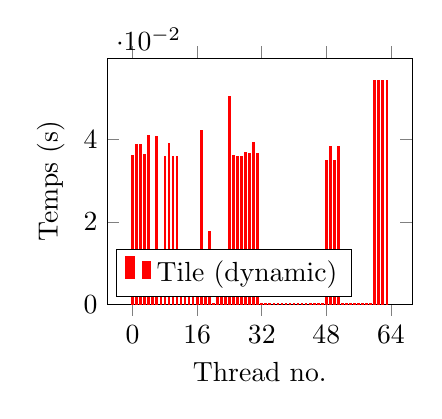
\begin{tikzpicture}
\begin{axis}[
  ybar,
  bar width=0.02cm,
  xlabel={Thread no.},
  ylabel={Temps (s)},
  ymin=0,
  legend pos=south west,
  width=0.45\textwidth,
  xtick distance=16
]

% Données pour le deuxième graphique (au milieu)
\addplot[color=red, fill=red] coordinates {
  (0,0.036062) (1,0.038855) (2,0.038824) (3,0.036425) (4,0.040986) (5,0.003205) (6,0.040622) (7,0.003470) (8,0.035948) (9,0.038930) (10,0.035934) (11,0.035987) (12,0.002953) (13,0.002935) (14,0.002888) (15,0.002948) (16,0.003841) (17,0.042303) (18,0.003923) (19,0.017662) (20,0.000070) (21,0.003971) (22,0.003608) (23,0.003937) (24,0.050465) (25,0.036109) (26,0.035929) (27,0.035843) (28,0.036849) (29,0.036650) (30,0.039241) (31,0.036651) (32,0.000071) (33,0.000071) (34,0.000071) (35,0.000072) (36,0.000075) (37,0.000072) (38,0.000072) (39,0.000072) (40,0.000075) (41,0.000075) (42,0.000075) (43,0.000075) (44,0.000073) (45,0.000073) (46,0.000073) (47,0.000071) (48,0.034894) (49,0.038253) (50,0.034884) (51,0.038382) (52,0.000077) (53,0.000077) (54,0.000077) (55,0.000077) (56,0.000077) (57,0.000077) (58,0.000077) (59,0.000077) (60,0.054364) (61,0.054347) (62,0.054356) (63,0.054365)
};
\addlegendentry{Tile (dynamic)}

\end{axis}
\end{tikzpicture}
\hfill
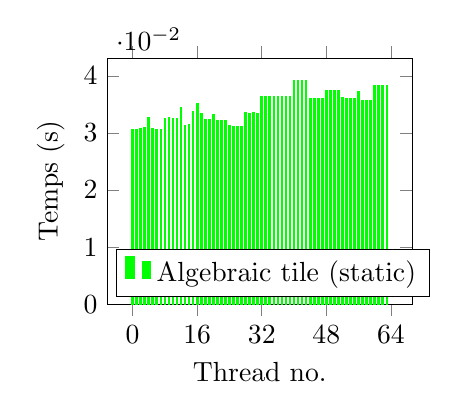
\begin{tikzpicture}
\begin{axis}[
  ybar,
  bar width=0.02cm,
  xlabel={Thread no.},
  ylabel={Temps (s)},
  ymin=0,
  legend pos=south west,
  width=0.45\textwidth,
  xtick distance=16
]

% Données pour le troisième graphique (à droite)
\addplot[color=green, fill=green] coordinates {
  (0,0.030602) (1,0.030621) (2,0.030827) (3,0.030993) (4,0.032704) (5,0.030819) (6,0.030604) (7,0.030613) (8,0.032554) (9,0.032624) (10,0.032574) (11,0.032563) (12,0.034500) (13,0.031374) (14,0.031392) (15,0.033806) (16,0.035144) (17,0.033341) (18,0.032402) (19,0.032289) (20,0.033183) (21,0.032219) (22,0.032170) (23,0.032183) (24,0.031226) (25,0.031208) (26,0.031192) (27,0.031197) (28,0.033491) (29,0.033480) (30,0.033502) (31,0.033488) (32,0.036360) (33,0.036339) (34,0.036334) (35,0.036338) (36,0.036417) (37,0.036370) (38,0.036400) (39,0.036395) (40,0.039193) (41,0.039165) (42,0.039172) (43,0.039186) (44,0.036028) (45,0.036013) (46,0.036026) (47,0.036018) (48,0.037452) (49,0.037362) (50,0.037361) (51,0.037437) (52,0.036264) (53,0.036106) (54,0.036054) (55,0.036060) (56,0.037228) (57,0.035648) (58,0.035643) (59,0.035644) (60,0.038325) (61,0.038280) (62,0.038243) (63,0.038304)
};
\addlegendentry{Algebraic tile (static)}

\end{axis}
\end{tikzpicture}

\caption{Temps d'exécution des threads pour le fichier trmm.c}
\label{fig:graphes}
\end{figure}

\begin{table}[htbp]
  \centering
  \caption{Statistiques pour le fichier trmm.c}
  \begin{tabular}{|c|c|c|c|}
    \hline
    Statistique & Algebraic Tile & Tile (static) & Tile (dynamic) \\ 
    \hline
    Skewness (g1)  & 0.0205686 & 0.315086 & 0.439243 \\ 
    Kurtosis (g2)  & -1.27302 & -1.88142 & -1.52346 \\ 
    Coefficient de variation $ \frac{\sigma}{\overline{x}} $ & 0.0767593 & 1.14854 & 1.10356\\ 
    Percent Imbalance metric en \% & 13.2926 & 152.182 & 202.645\\ 
    Coefficient de Gini  & 0.0437988 & 0.579325 & 0.580859\\ 
    Temps d'exécution (s) &  0.039254    &  0.040396   &  0.054570   \\ 

    \hline
  \end{tabular}
\end{table}
g1=$ \frac{\sum_{i=1}^{n} (x_i - \overline{x})^3}{n\sigma^3} $\
g2=$ \frac{\sum_{i=1}^{n} (x_i - \overline{x})^4}{n\sigma^4} $\
Coefficient de Gini = $ \frac{\sum_{i=1}^{n}\sum_{j=1}^{n} |x_i - x_j|}{2n^2\overline{x}} $\
\newpage

\begin{figure}
\centering

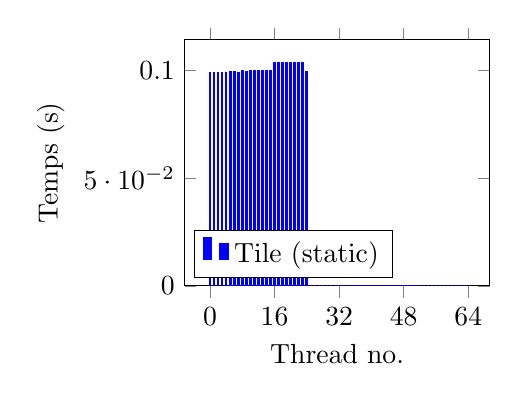
\begin{tikzpicture}
\begin{axis}[
  ybar,
  bar width=0.02cm,
  xlabel={Thread no.},
  ylabel={Temps (s)},
  ymin=0,
  legend pos=south west,
  width=0.45\textwidth,
  xtick distance=16
]

% Données pour le premier graphique (à gauche)
\addplot[color=blue, fill=blue] coordinates {
  (0,0.099116) (1,0.099072) (2,0.099080) (3,0.099054) (4,0.099119) (5,0.099170) (6,0.099179) (7,0.099134) (8,0.099705) (9,0.099528) (10,0.099664) (11,0.099703) (12,0.099862) (13,0.099811) (14,0.099843) (15,0.099852) (16,0.103667) (17,0.103596) (18,0.103582) (19,0.103617) (20,0.103762) (21,0.103743) (22,0.103713) (23,0.103727) (24,0.099433) (25,0.000056) (26,0.000056) (27,0.000057) (28,0.000054) (29,0.000055) (30,0.000055) (31,0.000054) (32,0.000057) (33,0.000057) (34,0.000057) (35,0.000057) (36,0.000056) (37,0.000056) (38,0.000056) (39,0.000056) (40,0.000055) (41,0.000055) (42,0.000055) (43,0.000055) (44,0.000057) (45,0.000057) (46,0.000057) (47,0.000057) (48,0.000056) (49,0.000056) (50,0.000056) (51,0.000056) (52,0.000058) (53,0.000058) (54,0.000058) (55,0.000058) (56,0.000058) (57,0.000058) (58,0.000058) (59,0.000058) (60,0.000057) (61,0.000057) (62,0.000057) (63,0.000057)
};
\addlegendentry{Tile (static)}

\end{axis}
\end{tikzpicture}
\hfill
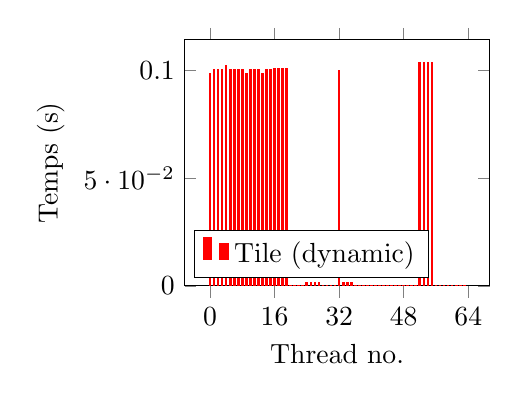
\begin{tikzpicture}
\begin{axis}[
  ybar,
  bar width=0.02cm,
  xlabel={Thread no.},
  ylabel={Temps (s)},
  ymin=0,
  legend pos=south west,
  width=0.45\textwidth,
  xtick distance=16
]

% Données pour le deuxième graphique (au milieu)
\addplot[color=red, fill=red] coordinates {
  (0,0.098512) (1,0.100282) (2,0.100251) (3,0.100266) (4,0.102197) (5,0.100485) (6,0.100440) (7,0.100416) (8,0.100209) (9,0.098560) (10,0.100240) (11,0.100231) (12,0.100298) (13,0.098520) (14,0.100305) (15,0.100328) (16,0.100718) (17,0.100738) (18,0.100738) (19,0.100708) (20,0.000063) (21,0.000063) (22,0.000063) (23,0.000063) (24,0.001716) (25,0.001678) (26,0.001698) (27,0.001680) (28,0.000064) (29,0.000063) (30,0.000063) (31,0.000062) (32,0.099859) (33,0.001516) (34,0.001554) (35,0.001534) (36,0.000067) (37,0.000068) (38,0.000068) (39,0.000067) (40,0.000066) (41,0.000066) (42,0.000066) (43,0.000066) (44,0.000068) (45,0.000068) (46,0.000068) (47,0.000068) (48,0.000063) (49,0.000063) (50,0.000063) (51,0.000063) (52,0.103862) (53,0.103873) (54,0.103835) (55,0.103833) (56,0.000065) (57,0.000065) (58,0.000064) (59,0.000065) (60,0.000066) (61,0.000066) (62,0.000066) (63,0.000066)
};
\addlegendentry{Tile (dynamic)}

\end{axis}
\end{tikzpicture}
\hfill
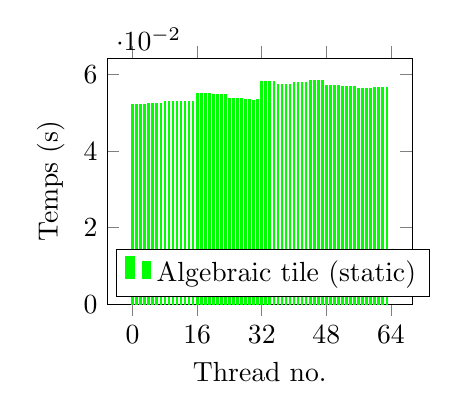
\begin{tikzpicture}
\begin{axis}[
  ybar,
  bar width=0.02cm,
  xlabel={Thread no.},
  ylabel={Temps (s)},
  ymin=0,
  legend pos=south west,
  width=0.45\textwidth,
  xtick distance=16
]

% Données pour le troisième graphique (à droite)
\addplot[color=green, fill=green] coordinates {
  (0,0.052208) (1,0.052199) (2,0.052277) (3,0.052267) (4,0.052484) (5,0.052467) (6,0.052503) (7,0.052498) (8,0.052896) (9,0.052869) (10,0.052888) (11,0.052923) (12,0.052904) (13,0.052908) (14,0.052905) (15,0.052893) (16,0.055023) (17,0.055017) (18,0.055021) (19,0.055016) (20,0.054909) (21,0.054921) (22,0.054856) (23,0.054911) (24,0.053750) (25,0.053755) (26,0.053756) (27,0.053741) (28,0.053398) (29,0.053429) (30,0.053375) (31,0.053409) (32,0.058310) (33,0.058265) (34,0.058274) (35,0.058285) (36,0.057347) (37,0.057362) (38,0.057353) (39,0.057343) (40,0.058046) (41,0.058077) (42,0.058066) (43,0.058087) (44,0.058499) (45,0.058482) (46,0.058494) (47,0.058474) (48,0.057218) (49,0.057186) (50,0.057192) (51,0.057195) (52,0.056905) (53,0.056878) (54,0.056900) (55,0.056897) (56,0.056449) (57,0.056421) (58,0.056432) (59,0.056427) (60,0.056706) (61,0.056656) (62,0.056617) (63,0.056670)
};
\addlegendentry{Algebraic tile (static)}

\end{axis}
\end{tikzpicture}

\caption{Temps d'exécution des threads pour le fichier 2mm.c}
\label{fig:graphes}
\end{figure}

\begin{table}[htbp]
  \centering
  \caption{Statistiques pour le fichier 2mm.c}
  \begin{tabular}{|c|c|c|c|}
    \hline
    Statistique & Algebraic Tile & Tile (static) & Tile (dynamic) \\ 
    \hline
    Skewness (g1)  & -0.0998966 & 0.45036 & 0.44926 \\ 
    Kurtosis (g2)  & -1.52083 & -1.79439 & -1.79615 \\ 
    Coefficient de variation $ \frac{\sigma}{\overline{x}} $ & 0.0390526 & 1.24761 & 1.2384\\ 
    Percent Imbalance metric en \% & 5.52567 & 163.321 & 162.433\\ 
    Coefficient de Gini  & 0.0222087 & 0.612413 & 0.609187\\ 
    Temps d'exécution (s) &  0.059578    &  0.104013   &  0.105760   \\ 

    \hline
  \end{tabular}
\end{table}
g1=$ \frac{\sum_{i=1}^{n} (x_i - \overline{x})^3}{n\sigma^3} $\
g2=$ \frac{\sum_{i=1}^{n} (x_i - \overline{x})^4}{n\sigma^4} $\
Coefficient de Gini = $ \frac{\sum_{i=1}^{n}\sum_{j=1}^{n} |x_i - x_j|}{2n^2\overline{x}} $\
\newpage

\begin{figure}
\centering

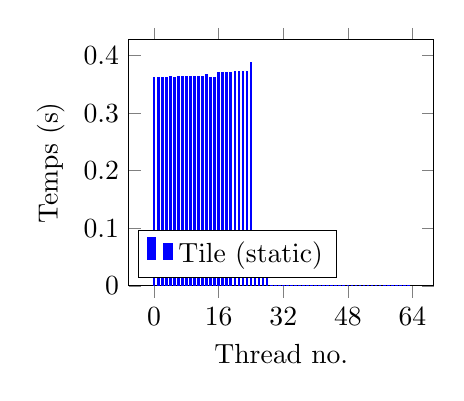
\begin{tikzpicture}
\begin{axis}[
  ybar,
  bar width=0.02cm,
  xlabel={Thread no.},
  ylabel={Temps (s)},
  ymin=0,
  legend pos=south west,
  width=0.45\textwidth,
  xtick distance=16
]

% Données pour le premier graphique (à gauche)
\addplot[color=blue, fill=blue] coordinates {
  (0,0.362637) (1,0.362334) (2,0.362423) (3,0.362444) (4,0.363464) (5,0.362511) (6,0.362913) (7,0.363018) (8,0.364362) (9,0.363293) (10,0.363502) (11,0.364344) (12,0.363739) (13,0.367228) (14,0.361931) (15,0.362182) (16,0.370087) (17,0.370203) (18,0.370312) (19,0.370182) (20,0.372217) (21,0.371862) (22,0.371915) (23,0.371897) (24,0.388771) (25,0.074414) (26,0.074402) (27,0.074371) (28,0.025401) (29,0.000099) (30,0.000099) (31,0.000099) (32,0.000103) (33,0.000103) (34,0.000103) (35,0.000103) (36,0.000105) (37,0.000105) (38,0.000105) (39,0.000105) (40,0.000106) (41,0.000106) (42,0.000106) (43,0.000106) (44,0.000106) (45,0.000106) (46,0.000106) (47,0.000106) (48,0.000095) (49,0.000095) (50,0.000095) (51,0.000095) (52,0.000102) (53,0.000101) (54,0.000100) (55,0.000100) (56,0.000104) (57,0.000104) (58,0.000104) (59,0.000104) (60,0.000104) (61,0.000104) (62,0.000104) (63,0.000104)
};
\addlegendentry{Tile (static)}

\end{axis}
\end{tikzpicture}
\hfill
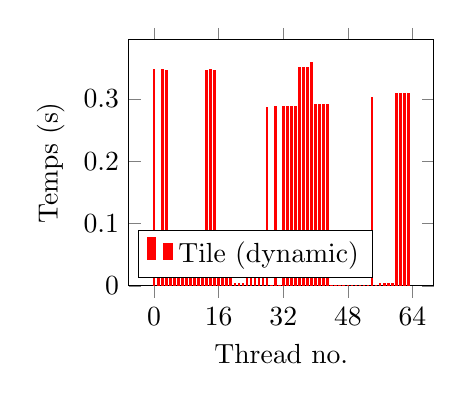
\begin{tikzpicture}
\begin{axis}[
  ybar,
  bar width=0.02cm,
  xlabel={Thread no.},
  ylabel={Temps (s)},
  ymin=0,
  legend pos=south west,
  width=0.45\textwidth,
  xtick distance=16
]

% Données pour le deuxième graphique (au milieu)
\addplot[color=red, fill=red] coordinates {
  (0,0.346313) (1,0.060592) (2,0.346409) (3,0.345827) (4,0.063056) (5,0.063645) (6,0.063947) (7,0.063793) (8,0.063108) (9,0.062921) (10,0.063236) (11,0.063189) (12,0.060507) (13,0.344688) (14,0.346280) (15,0.345191) (16,0.075986) (17,0.075981) (18,0.075999) (19,0.075915) (20,0.004102) (21,0.004069) (22,0.004091) (23,0.034962) (24,0.083744) (25,0.083753) (26,0.085225) (27,0.083727) (28,0.286720) (29,0.001155) (30,0.286966) (31,0.001149) (32,0.287904) (33,0.288025) (34,0.288082) (35,0.287915) (36,0.350307) (37,0.350305) (38,0.350306) (39,0.358850) (40,0.290541) (41,0.290516) (42,0.290494) (43,0.290513) (44,0.000123) (45,0.000123) (46,0.000124) (47,0.000123) (48,0.001166) (49,0.001179) (50,0.001145) (51,0.001004) (52,0.000120) (53,0.000121) (54,0.302015) (55,0.000121) (56,0.003039) (57,0.003099) (58,0.003115) (59,0.003113) (60,0.308718) (61,0.308711) (62,0.308719) (63,0.308695)
};
\addlegendentry{Tile (dynamic)}

\end{axis}
\end{tikzpicture}
\hfill
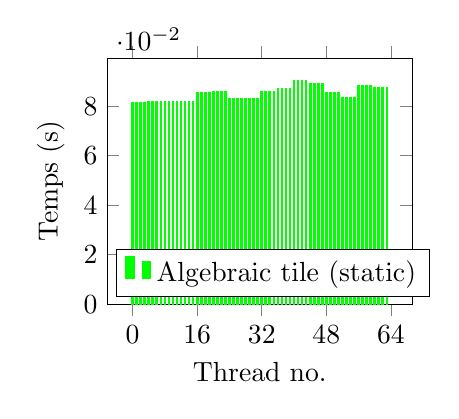
\begin{tikzpicture}
\begin{axis}[
  ybar,
  bar width=0.02cm,
  xlabel={Thread no.},
  ylabel={Temps (s)},
  ymin=0,
  legend pos=south west,
  width=0.45\textwidth,
  xtick distance=16
]

% Données pour le troisième graphique (à droite)
\addplot[color=green, fill=green] coordinates {
  (0,0.081329) (1,0.081327) (2,0.081399) (3,0.081449) (4,0.081770) (5,0.081765) (6,0.081833) (7,0.081834) (8,0.081888) (9,0.081920) (10,0.081980) (11,0.081949) (12,0.081847) (13,0.081822) (14,0.081926) (15,0.081897) (16,0.085615) (17,0.085626) (18,0.085623) (19,0.085673) (20,0.085741) (21,0.085873) (22,0.085869) (23,0.085916) (24,0.083018) (25,0.082924) (26,0.083141) (27,0.083126) (28,0.083050) (29,0.083142) (30,0.083194) (31,0.083113) (32,0.085880) (33,0.085823) (34,0.085816) (35,0.085816) (36,0.086941) (37,0.086987) (38,0.087023) (39,0.087013) (40,0.090341) (41,0.090293) (42,0.090365) (43,0.090374) (44,0.089043) (45,0.089126) (46,0.089109) (47,0.089077) (48,0.085631) (49,0.085682) (50,0.085621) (51,0.085673) (52,0.083493) (53,0.083551) (54,0.083477) (55,0.083545) (56,0.088213) (57,0.088224) (58,0.088208) (59,0.088231) (60,0.087568) (61,0.087505) (62,0.087442) (63,0.087539)
};
\addlegendentry{Algebraic tile (static)}

\end{axis}
\end{tikzpicture}

\caption{Temps d'exécution des threads pour le fichier 3mm.c}
\label{fig:graphes}
\end{figure}

\begin{table}[htbp]
  \centering
  \caption{Statistiques pour le fichier 3mm.c}
  \begin{tabular}{|c|c|c|c|}
    \hline
    Statistique & Algebraic Tile & Tile (static) & Tile (dynamic) \\ 
    \hline
    Skewness (g1)  & 0.249757 & 0.428384 & 0.385039 \\ 
    Kurtosis (g2)  & -1.10492 & -1.79218 & -1.65519 \\ 
    Coefficient de variation $ \frac{\sigma}{\overline{x}} $ & 0.0321818 & 1.19911 & 0.978075\\ 
    Percent Imbalance metric en \% & 6.18169 & 164.078 & 148.43\\ 
    Coefficient de Gini  & 0.0182602 & 0.600141 & 0.527851\\ 
    Temps d'exécution (s) &  0.090851    &  0.389385   &  0.391218   \\ 

    \hline
  \end{tabular}
\end{table}
g1=$ \frac{\sum_{i=1}^{n} (x_i - \overline{x})^3}{n\sigma^3} $\
g2=$ \frac{\sum_{i=1}^{n} (x_i - \overline{x})^4}{n\sigma^4} $\
Coefficient de Gini = $ \frac{\sum_{i=1}^{n}\sum_{j=1}^{n} |x_i - x_j|}{2n^2\overline{x}} $\
\newpage

\begin{figure}
\centering

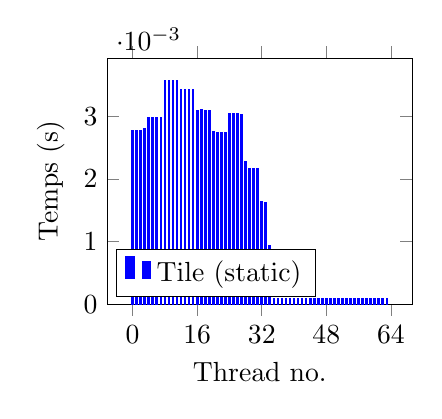
\begin{tikzpicture}
\begin{axis}[
  ybar,
  bar width=0.02cm,
  xlabel={Thread no.},
  ylabel={Temps (s)},
  ymin=0,
  legend pos=south west,
  width=0.45\textwidth,
  xtick distance=16
]

% Données pour le premier graphique (à gauche)
\addplot[color=blue, fill=blue] coordinates {
  (0,0.002773) (1,0.002766) (2,0.002775) (3,0.002801) (4,0.002984) (5,0.002981) (6,0.002982) (7,0.002982) (8,0.003573) (9,0.003566) (10,0.003567) (11,0.003569) (12,0.003428) (13,0.003429) (14,0.003430) (15,0.003427) (16,0.003097) (17,0.003102) (18,0.003094) (19,0.003091) (20,0.002757) (21,0.002740) (22,0.002748) (23,0.002747) (24,0.003038) (25,0.003039) (26,0.003039) (27,0.003036) (28,0.002283) (29,0.002163) (30,0.002163) (31,0.002163) (32,0.001638) (33,0.001627) (34,0.000937) (35,0.000088) (36,0.000088) (37,0.000088) (38,0.000087) (39,0.000087) (40,0.000088) (41,0.000089) (42,0.000089) (43,0.000089) (44,0.000091) (45,0.000088) (46,0.000089) (47,0.000088) (48,0.000091) (49,0.000088) (50,0.000087) (51,0.000087) (52,0.000088) (53,0.000088) (54,0.000088) (55,0.000088) (56,0.000089) (57,0.000088) (58,0.000087) (59,0.000087) (60,0.000089) (61,0.000089) (62,0.000087) (63,0.000087)
};
\addlegendentry{Tile (static)}

\end{axis}
\end{tikzpicture}
\hfill
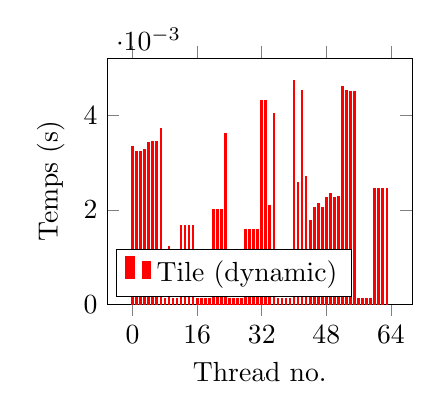
\begin{tikzpicture}
\begin{axis}[
  ybar,
  bar width=0.02cm,
  xlabel={Thread no.},
  ylabel={Temps (s)},
  ymin=0,
  legend pos=south west,
  width=0.45\textwidth,
  xtick distance=16
]

% Données pour le deuxième graphique (au milieu)
\addplot[color=red, fill=red] coordinates {
  (0,0.003335) (1,0.003243) (2,0.003225) (3,0.003269) (4,0.003424) (5,0.003456) (6,0.003455) (7,0.003715) (8,0.000125) (9,0.001228) (10,0.000126) (11,0.000125) (12,0.001656) (13,0.001660) (14,0.001657) (15,0.001658) (16,0.000115) (17,0.000116) (18,0.000116) (19,0.000120) (20,0.002009) (21,0.002012) (22,0.002011) (23,0.003626) (24,0.000123) (25,0.000121) (26,0.000121) (27,0.000121) (28,0.001571) (29,0.001571) (30,0.001571) (31,0.001571) (32,0.004318) (33,0.004321) (34,0.002091) (35,0.004049) (36,0.000121) (37,0.000118) (38,0.000124) (39,0.000118) (40,0.004741) (41,0.002579) (42,0.004529) (43,0.002710) (44,0.001782) (45,0.002038) (46,0.002123) (47,0.002055) (48,0.002265) (49,0.002337) (50,0.002267) (51,0.002283) (52,0.004620) (53,0.004534) (54,0.004504) (55,0.004498) (56,0.000115) (57,0.000115) (58,0.000115) (59,0.000115) (60,0.002457) (61,0.002457) (62,0.002457) (63,0.002457)
};
\addlegendentry{Tile (dynamic)}

\end{axis}
\end{tikzpicture}
\hfill
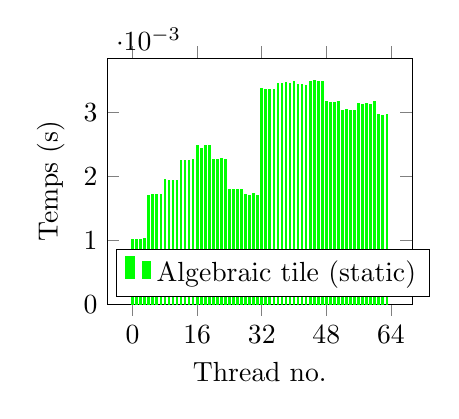
\begin{tikzpicture}
\begin{axis}[
  ybar,
  bar width=0.02cm,
  xlabel={Thread no.},
  ylabel={Temps (s)},
  ymin=0,
  legend pos=south west,
  width=0.45\textwidth,
  xtick distance=16
]

% Données pour le troisième graphique (à droite)
\addplot[color=green, fill=green] coordinates {
  (0,0.001011) (1,0.001011) (2,0.001013) (3,0.001023) (4,0.001707) (5,0.001708) (6,0.001714) (7,0.001718) (8,0.001944) (9,0.001938) (10,0.001936) (11,0.001941) (12,0.002249) (13,0.002246) (14,0.002253) (15,0.002257) (16,0.002477) (17,0.002438) (18,0.002485) (19,0.002477) (20,0.002267) (21,0.002269) (22,0.002279) (23,0.002269) (24,0.001794) (25,0.001787) (26,0.001791) (27,0.001788) (28,0.001713) (29,0.001706) (30,0.001732) (31,0.001705) (32,0.003377) (33,0.003357) (34,0.003355) (35,0.003355) (36,0.003458) (37,0.003455) (38,0.003461) (39,0.003458) (40,0.003482) (41,0.003436) (42,0.003435) (43,0.003422) (44,0.003480) (45,0.003501) (46,0.003479) (47,0.003486) (48,0.003176) (49,0.003148) (50,0.003158) (51,0.003169) (52,0.003029) (53,0.003046) (54,0.003026) (55,0.003031) (56,0.003140) (57,0.003123) (58,0.003142) (59,0.003118) (60,0.003168) (61,0.002962) (62,0.002951) (63,0.002967)
};
\addlegendentry{Algebraic tile (static)}

\end{axis}
\end{tikzpicture}

\caption{Temps d'exécution des threads pour le fichier atax.c}
\label{fig:graphes}
\end{figure}

\begin{table}[htbp]
  \centering
  \caption{Statistiques pour le fichier atax.c}
  \begin{tabular}{|c|c|c|c|}
    \hline
    Statistique & Algebraic Tile & Tile (static) & Tile (dynamic) \\ 
    \hline
    Skewness (g1)  & -0.403754 & 0.0298462 & 0.177939 \\ 
    Kurtosis (g2)  & -1.07236 & -1.82441 & -1.09292 \\ 
    Coefficient de variation $ \frac{\sigma}{\overline{x}} $ & 0.294088 & 0.902726 & 0.752037\\ 
    Percent Imbalance metric en \% & 35.7987 & 123.986 & 137.672\\ 
    Coefficient de Gini  & 0.165077 & 0.48603 & 0.424612\\ 
    Temps d'exécution (s) &  0.003573    &  0.003638   &  0.004914   \\ 

    \hline
  \end{tabular}
\end{table}
g1=$ \frac{\sum_{i=1}^{n} (x_i - \overline{x})^3}{n\sigma^3} $\
g2=$ \frac{\sum_{i=1}^{n} (x_i - \overline{x})^4}{n\sigma^4} $\
Coefficient de Gini = $ \frac{\sum_{i=1}^{n}\sum_{j=1}^{n} |x_i - x_j|}{2n^2\overline{x}} $\
\newpage

\begin{figure}
\centering

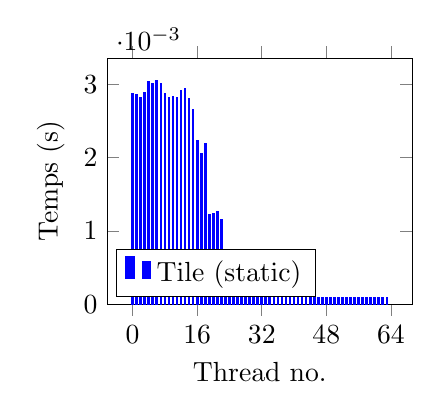
\begin{tikzpicture}
\begin{axis}[
  ybar,
  bar width=0.02cm,
  xlabel={Thread no.},
  ylabel={Temps (s)},
  ymin=0,
  legend pos=south west,
  width=0.45\textwidth,
  xtick distance=16
]

% Données pour le premier graphique (à gauche)
\addplot[color=blue, fill=blue] coordinates {
  (0,0.002876) (1,0.002861) (2,0.002821) (3,0.002883) (4,0.003034) (5,0.003009) (6,0.003050) (7,0.003009) (8,0.002878) (9,0.002812) (10,0.002834) (11,0.002815) (12,0.002918) (13,0.002934) (14,0.002797) (15,0.002659) (16,0.002230) (17,0.002060) (18,0.002196) (19,0.001224) (20,0.001239) (21,0.001268) (22,0.001153) (23,0.000086) (24,0.000086) (25,0.000085) (26,0.000085) (27,0.000086) (28,0.000085) (29,0.000086) (30,0.000085) (31,0.000085) (32,0.000089) (33,0.000090) (34,0.000089) (35,0.000090) (36,0.000091) (37,0.000091) (38,0.000091) (39,0.000091) (40,0.000092) (41,0.000092) (42,0.000092) (43,0.000092) (44,0.000092) (45,0.000091) (46,0.000091) (47,0.000091) (48,0.000086) (49,0.000087) (50,0.000086) (51,0.000086) (52,0.000088) (53,0.000088) (54,0.000088) (55,0.000088) (56,0.000089) (57,0.000089) (58,0.000089) (59,0.000089) (60,0.000089) (61,0.000089) (62,0.000089) (63,0.000089)
};
\addlegendentry{Tile (static)}

\end{axis}
\end{tikzpicture}
\hfill
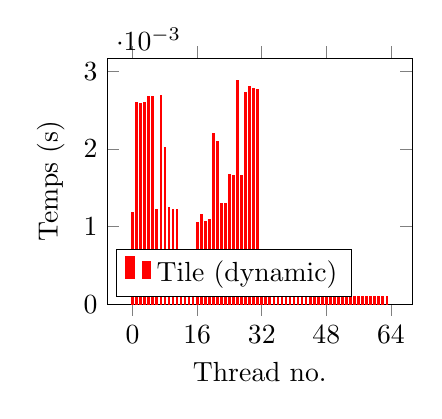
\begin{tikzpicture}
\begin{axis}[
  ybar,
  bar width=0.02cm,
  xlabel={Thread no.},
  ylabel={Temps (s)},
  ymin=0,
  legend pos=south west,
  width=0.45\textwidth,
  xtick distance=16
]

% Données pour le deuxième graphique (au milieu)
\addplot[color=red, fill=red] coordinates {
  (0,0.001180) (1,0.002595) (2,0.002585) (3,0.002597) (4,0.002676) (5,0.002675) (6,0.001218) (7,0.002693) (8,0.002016) (9,0.001240) (10,0.001220) (11,0.001225) (12,0.000104) (13,0.000106) (14,0.000104) (15,0.000104) (16,0.001050) (17,0.001160) (18,0.001067) (19,0.001091) (20,0.002204) (21,0.002091) (22,0.001301) (23,0.001303) (24,0.001665) (25,0.001662) (26,0.002883) (27,0.001658) (28,0.002731) (29,0.002811) (30,0.002784) (31,0.002761) (32,0.000113) (33,0.000109) (34,0.000103) (35,0.000108) (36,0.000107) (37,0.000107) (38,0.000107) (39,0.000107) (40,0.000106) (41,0.000106) (42,0.000106) (43,0.000106) (44,0.000106) (45,0.000108) (46,0.000110) (47,0.000107) (48,0.000100) (49,0.000100) (50,0.000100) (51,0.000100) (52,0.000102) (53,0.000102) (54,0.000102) (55,0.000102) (56,0.000103) (57,0.000102) (58,0.000102) (59,0.000102) (60,0.000101) (61,0.000101) (62,0.000101) (63,0.000101)
};
\addlegendentry{Tile (dynamic)}

\end{axis}
\end{tikzpicture}
\hfill
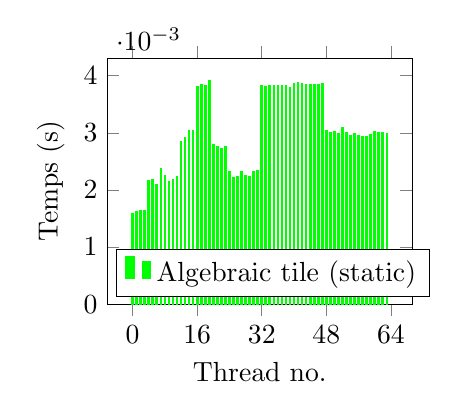
\begin{tikzpicture}
\begin{axis}[
  ybar,
  bar width=0.02cm,
  xlabel={Thread no.},
  ylabel={Temps (s)},
  ymin=0,
  legend pos=south west,
  width=0.45\textwidth,
  xtick distance=16
]

% Données pour le troisième graphique (à droite)
\addplot[color=green, fill=green] coordinates {
  (0,0.001580) (1,0.001615) (2,0.001631) (3,0.001637) (4,0.002159) (5,0.002178) (6,0.002098) (7,0.002374) (8,0.002256) (9,0.002141) (10,0.002175) (11,0.002231) (12,0.002841) (13,0.002925) (14,0.003043) (15,0.003046) (16,0.003815) (17,0.003843) (18,0.003824) (19,0.003916) (20,0.002798) (21,0.002761) (22,0.002721) (23,0.002757) (24,0.002319) (25,0.002223) (26,0.002238) (27,0.002317) (28,0.002248) (29,0.002236) (30,0.002328) (31,0.002344) (32,0.003822) (33,0.003809) (34,0.003823) (35,0.003832) (36,0.003821) (37,0.003827) (38,0.003825) (39,0.003796) (40,0.003861) (41,0.003872) (42,0.003870) (43,0.003849) (44,0.003844) (45,0.003841) (46,0.003838) (47,0.003860) (48,0.003034) (49,0.003013) (50,0.003025) (51,0.002985) (52,0.003089) (53,0.003010) (54,0.002960) (55,0.002988) (56,0.002957) (57,0.002943) (58,0.002942) (59,0.002965) (60,0.003016) (61,0.003008) (62,0.003007) (63,0.002986)
};
\addlegendentry{Algebraic tile (static)}

\end{axis}
\end{tikzpicture}

\caption{Temps d'exécution des threads pour le fichier bicg.c}
\label{fig:graphes}
\end{figure}

\begin{table}[htbp]
  \centering
  \caption{Statistiques pour le fichier bicg.c}
  \begin{tabular}{|c|c|c|c|}
    \hline
    Statistique & Algebraic Tile & Tile (static) & Tile (dynamic) \\ 
    \hline
    Skewness (g1)  & -0.136187 & 0.814057 & 0.798409 \\ 
    Kurtosis (g2)  & -1.05569 & -1.19965 & -0.932481 \\ 
    Coefficient de variation $ \frac{\sigma}{\overline{x}} $ & 0.235625 & 1.27643 & 1.12203\\ 
    Percent Imbalance metric en \% & 31.9518 & 218.991 & 218.69\\ 
    Coefficient de Gini  & 0.13188 & 0.624598 & 0.579447\\ 
    Temps d'exécution (s) &  0.003997    &  0.003164   &  0.002941   \\ 

    \hline
  \end{tabular}
\end{table}
g1=$ \frac{\sum_{i=1}^{n} (x_i - \overline{x})^3}{n\sigma^3} $\
g2=$ \frac{\sum_{i=1}^{n} (x_i - \overline{x})^4}{n\sigma^4} $\
Coefficient de Gini = $ \frac{\sum_{i=1}^{n}\sum_{j=1}^{n} |x_i - x_j|}{2n^2\overline{x}} $\
\newpage

\begin{figure}
\centering

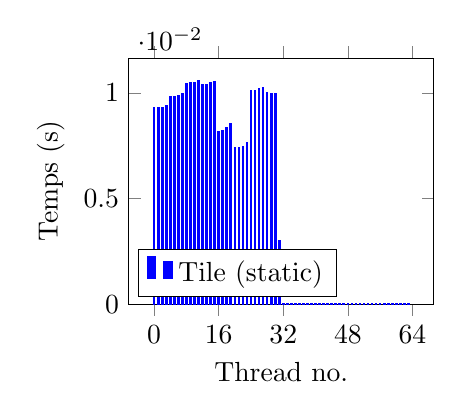
\begin{tikzpicture}
\begin{axis}[
  ybar,
  bar width=0.02cm,
  xlabel={Thread no.},
  ylabel={Temps (s)},
  ymin=0,
  legend pos=south west,
  width=0.45\textwidth,
  xtick distance=16
]

% Données pour le premier graphique (à gauche)
\addplot[color=blue, fill=blue] coordinates {
  (0,0.009324) (1,0.009324) (2,0.009325) (3,0.009388) (4,0.009833) (5,0.009833) (6,0.009856) (7,0.009956) (8,0.010452) (9,0.010483) (10,0.010514) (11,0.010588) (12,0.010407) (13,0.010407) (14,0.010477) (15,0.010553) (16,0.008170) (17,0.008200) (18,0.008345) (19,0.008545) (20,0.007419) (21,0.007419) (22,0.007480) (23,0.007642) (24,0.010096) (25,0.010134) (26,0.010186) (27,0.010241) (28,0.010009) (29,0.009980) (30,0.009971) (31,0.003001) (32,0.000033) (33,0.000033) (34,0.000033) (35,0.000033) (36,0.000033) (37,0.000033) (38,0.000033) (39,0.000033) (40,0.000034) (41,0.000034) (42,0.000034) (43,0.000034) (44,0.000034) (45,0.000034) (46,0.000034) (47,0.000034) (48,0.000032) (49,0.000032) (50,0.000032) (51,0.000032) (52,0.000033) (53,0.000033) (54,0.000033) (55,0.000033) (56,0.000034) (57,0.000034) (58,0.000034) (59,0.000034) (60,0.000034) (61,0.000034) (62,0.000034) (63,0.000033)
};
\addlegendentry{Tile (static)}

\end{axis}
\end{tikzpicture}
\hfill
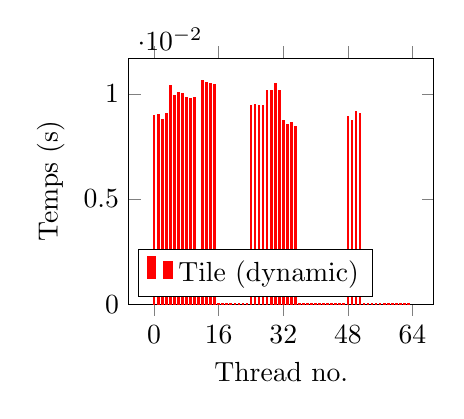
\begin{tikzpicture}
\begin{axis}[
  ybar,
  bar width=0.02cm,
  xlabel={Thread no.},
  ylabel={Temps (s)},
  ymin=0,
  legend pos=south west,
  width=0.45\textwidth,
  xtick distance=16
]

% Données pour le deuxième graphique (au milieu)
\addplot[color=red, fill=red] coordinates {
  (0,0.008982) (1,0.009031) (2,0.008759) (3,0.009059) (4,0.010383) (5,0.009934) (6,0.010061) (7,0.010020) (8,0.009825) (9,0.009788) (10,0.009818) (11,0.002478) (12,0.010637) (13,0.010527) (14,0.010468) (15,0.010421) (16,0.000041) (17,0.000041) (18,0.000041) (19,0.000041) (20,0.000041) (21,0.000042) (22,0.000041) (23,0.000041) (24,0.009423) (25,0.009504) (26,0.009430) (27,0.009426) (28,0.010136) (29,0.010136) (30,0.010482) (31,0.010178) (32,0.008732) (33,0.008523) (34,0.008637) (35,0.008434) (36,0.000042) (37,0.000042) (38,0.000042) (39,0.000042) (40,0.000042) (41,0.000042) (42,0.000042) (43,0.000042) (44,0.000043) (45,0.000043) (46,0.000043) (47,0.000043) (48,0.008913) (49,0.008712) (50,0.009152) (51,0.009067) (52,0.000043) (53,0.000043) (54,0.000043) (55,0.000043) (56,0.000040) (57,0.000040) (58,0.000040) (59,0.000040) (60,0.000041) (61,0.000040) (62,0.000041) (63,0.000040)
};
\addlegendentry{Tile (dynamic)}

\end{axis}
\end{tikzpicture}
\hfill
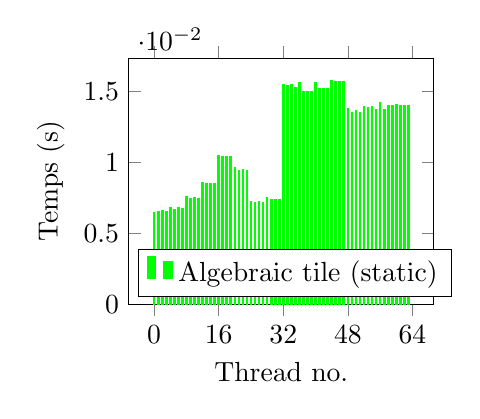
\begin{tikzpicture}
\begin{axis}[
  ybar,
  bar width=0.02cm,
  xlabel={Thread no.},
  ylabel={Temps (s)},
  ymin=0,
  legend pos=south west,
  width=0.45\textwidth,
  xtick distance=16
]

% Données pour le troisième graphique (à droite)
\addplot[color=green, fill=green] coordinates {
  (0,0.006492) (1,0.006531) (2,0.006582) (3,0.006549) (4,0.006808) (5,0.006704) (6,0.006787) (7,0.006740) (8,0.007620) (9,0.007430) (10,0.007541) (11,0.007437) (12,0.008602) (13,0.008493) (14,0.008534) (15,0.008499) (16,0.010486) (17,0.010398) (18,0.010441) (19,0.010419) (20,0.009625) (21,0.009452) (22,0.009518) (23,0.009461) (24,0.007252) (25,0.007165) (26,0.007220) (27,0.007184) (28,0.007504) (29,0.007378) (30,0.007398) (31,0.007367) (32,0.015524) (33,0.015452) (34,0.015470) (35,0.015278) (36,0.015600) (37,0.015032) (38,0.015009) (39,0.015029) (40,0.015651) (41,0.015217) (42,0.015229) (43,0.015218) (44,0.015779) (45,0.015679) (46,0.015685) (47,0.015705) (48,0.013765) (49,0.013521) (50,0.013642) (51,0.013521) (52,0.013961) (53,0.013836) (54,0.013934) (55,0.013714) (56,0.014228) (57,0.013715) (58,0.013977) (59,0.013988) (60,0.014057) (61,0.014012) (62,0.014003) (63,0.014002)
};
\addlegendentry{Algebraic tile (static)}

\end{axis}
\end{tikzpicture}

\caption{Temps d'exécution des threads pour le fichier mvt.c}
\label{fig:graphes}
\end{figure}

\begin{table}[htbp]
  \centering
  \caption{Statistiques pour le fichier mvt.c}
  \begin{tabular}{|c|c|c|c|}
    \hline
    Statistique & Algebraic Tile & Tile (static) & Tile (dynamic) \\ 
    \hline
    Skewness (g1)  & -0.101443 & 0.111231 & 0.0813751 \\ 
    Kurtosis (g2)  & -1.71192 & -1.90608 & -1.9466 \\ 
    Coefficient de variation $ \frac{\sigma}{\overline{x}} $ & 0.308989 & 1.01917 & 1.01332\\ 
    Percent Imbalance metric en \% & 39.473 & 126.917 & 126.615\\ 
    Coefficient de Gini  & 0.172549 & 0.534795 & 0.526337\\ 
    Temps d'exécution (s) &  0.015902    &  0.010658   &  0.010737   \\ 

    \hline
  \end{tabular}
\end{table}
g1=$ \frac{\sum_{i=1}^{n} (x_i - \overline{x})^3}{n\sigma^3} $\
g2=$ \frac{\sum_{i=1}^{n} (x_i - \overline{x})^4}{n\sigma^4} $\
Coefficient de Gini = $ \frac{\sum_{i=1}^{n}\sum_{j=1}^{n} |x_i - x_j|}{2n^2\overline{x}} $\
\newpage

\begin{figure}
\centering

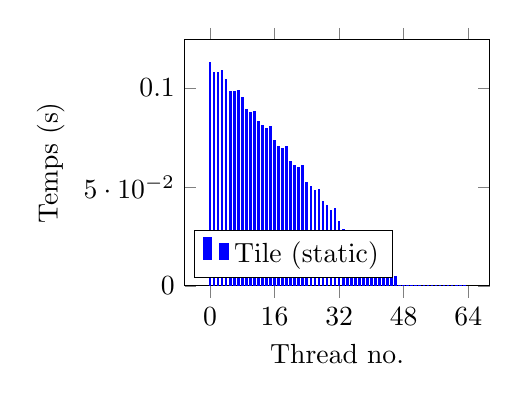
\begin{tikzpicture}
\begin{axis}[
  ybar,
  bar width=0.02cm,
  xlabel={Thread no.},
  ylabel={Temps (s)},
  ymin=0,
  legend pos=south west,
  width=0.45\textwidth,
  xtick distance=16
]

% Données pour le premier graphique (à gauche)
\addplot[color=blue, fill=blue] coordinates {
  (0,0.113066) (1,0.108020) (2,0.107718) (3,0.108628) (4,0.104040) (5,0.098109) (6,0.098107) (7,0.098643) (8,0.094938) (9,0.088961) (10,0.087598) (11,0.088301) (12,0.083134) (13,0.080808) (14,0.079497) (15,0.080249) (16,0.073364) (17,0.070134) (18,0.069326) (19,0.070211) (20,0.062636) (21,0.060633) (22,0.059968) (23,0.060607) (24,0.052424) (25,0.050272) (26,0.048233) (27,0.048798) (28,0.042360) (29,0.040553) (30,0.038169) (31,0.038969) (32,0.032569) (33,0.028259) (34,0.025565) (35,0.023823) (36,0.022129) (37,0.018884) (38,0.015669) (39,0.013827) (40,0.009680) (41,0.005067) (42,0.005060) (43,0.005061) (44,0.004842) (45,0.004840) (46,0.004657) (47,0.000209) (48,0.000201) (49,0.000201) (50,0.000201) (51,0.000201) (52,0.000204) (53,0.000204) (54,0.000204) (55,0.000204) (56,0.000204) (57,0.000204) (58,0.000204) (59,0.000204) (60,0.000208) (61,0.000209) (62,0.000208) (63,0.000208)
};
\addlegendentry{Tile (static)}

\end{axis}
\end{tikzpicture}
\hfill
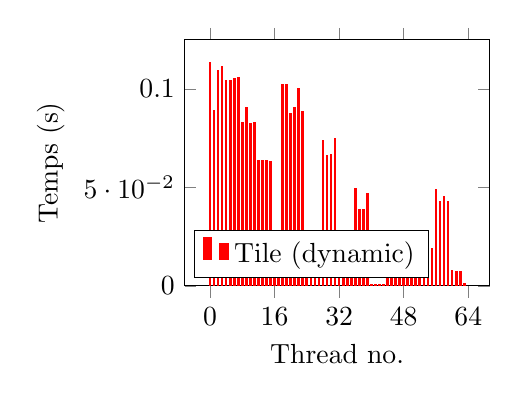
\begin{tikzpicture}
\begin{axis}[
  ybar,
  bar width=0.02cm,
  xlabel={Thread no.},
  ylabel={Temps (s)},
  ymin=0,
  legend pos=south west,
  width=0.45\textwidth,
  xtick distance=16
]

% Données pour le deuxième graphique (au milieu)
\addplot[color=red, fill=red] coordinates {
  (0,0.113588) (1,0.088950) (2,0.109093) (3,0.111541) (4,0.104244) (5,0.104194) (6,0.104995) (7,0.105542) (8,0.082660) (9,0.090766) (10,0.082636) (11,0.082742) (12,0.063467) (13,0.063512) (14,0.063498) (15,0.063282) (16,0.023808) (17,0.023876) (18,0.102075) (19,0.102000) (20,0.087254) (21,0.090392) (22,0.099931) (23,0.088524) (24,0.014639) (25,0.007395) (26,0.005581) (27,0.014591) (28,0.073543) (29,0.066265) (30,0.066701) (31,0.074973) (32,0.016322) (33,0.016712) (34,0.016631) (35,0.016505) (36,0.049486) (37,0.038512) (38,0.038541) (39,0.046893) (40,0.000880) (41,0.000814) (42,0.000651) (43,0.000705) (44,0.015796) (45,0.022076) (46,0.019477) (47,0.024370) (48,0.021965) (49,0.021957) (50,0.021981) (51,0.022051) (52,0.020587) (53,0.023138) (54,0.025630) (55,0.019037) (56,0.049006) (57,0.042987) (58,0.045520) (59,0.043002) (60,0.007504) (61,0.007400) (62,0.007431) (63,0.001311)
};
\addlegendentry{Tile (dynamic)}

\end{axis}
\end{tikzpicture}
\hfill
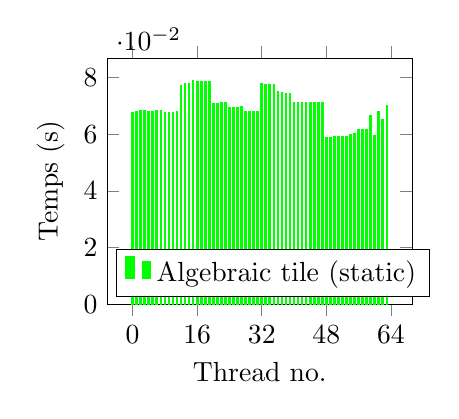
\begin{tikzpicture}
\begin{axis}[
  ybar,
  bar width=0.02cm,
  xlabel={Thread no.},
  ylabel={Temps (s)},
  ymin=0,
  legend pos=south west,
  width=0.45\textwidth,
  xtick distance=16
]

% Données pour le troisième graphique (à droite)
\addplot[color=green, fill=green] coordinates {
  (0,0.067811) (1,0.067971) (2,0.068203) (3,0.068382) (4,0.068117) (5,0.068181) (6,0.068237) (7,0.068291) (8,0.067730) (9,0.067626) (10,0.067816) (11,0.068151) (12,0.077311) (13,0.077874) (14,0.077893) (15,0.078984) (16,0.078665) (17,0.078786) (18,0.078762) (19,0.078583) (20,0.070842) (21,0.070970) (22,0.071031) (23,0.071269) (24,0.069393) (25,0.069294) (26,0.069309) (27,0.069760) (28,0.068171) (29,0.068037) (30,0.068008) (31,0.068131) (32,0.077766) (33,0.077660) (34,0.077651) (35,0.077661) (36,0.074925) (37,0.074557) (38,0.074515) (39,0.074474) (40,0.071065) (41,0.071038) (42,0.071090) (43,0.071103) (44,0.071119) (45,0.071067) (46,0.071067) (47,0.071128) (48,0.059005) (49,0.058936) (50,0.059116) (51,0.059073) (52,0.059020) (53,0.059106) (54,0.059863) (55,0.060270) (56,0.061619) (57,0.061664) (58,0.061648) (59,0.066505) (60,0.059394) (61,0.067858) (62,0.065191) (63,0.070285)
};
\addlegendentry{Algebraic tile (static)}

\end{axis}
\end{tikzpicture}

\caption{Temps d'exécution des threads pour le fichier correlation.c}
\label{fig:graphes}
\end{figure}

\begin{table}[htbp]
  \centering
  \caption{Statistiques pour le fichier correlation.c}
  \begin{tabular}{|c|c|c|c|}
    \hline
    Statistique & Algebraic Tile & Tile (static) & Tile (dynamic) \\ 
    \hline
    Skewness (g1)  & -0.182095 & 0.390587 & 0.370553 \\ 
    Kurtosis (g2)  & -0.653315 & -1.31771 & -1.31835 \\ 
    Coefficient de variation $ \frac{\sigma}{\overline{x}} $ & 0.0847962 & 0.933138 & 0.753317\\ 
    Percent Imbalance metric en \% & 13.7477 & 175.154 & 135.94\\ 
    Coefficient de Gini  & 0.0471739 & 0.523821 & 0.425959\\ 
    Temps d'exécution (s) &  0.084219    &  0.116218   &  0.125757   \\ 

    \hline
  \end{tabular}
\end{table}
g1=$ \frac{\sum_{i=1}^{n} (x_i - \overline{x})^3}{n\sigma^3} $\
g2=$ \frac{\sum_{i=1}^{n} (x_i - \overline{x})^4}{n\sigma^4} $\
Coefficient de Gini = $ \frac{\sum_{i=1}^{n}\sum_{j=1}^{n} |x_i - x_j|}{2n^2\overline{x}} $\
\newpage

\begin{figure}
\centering

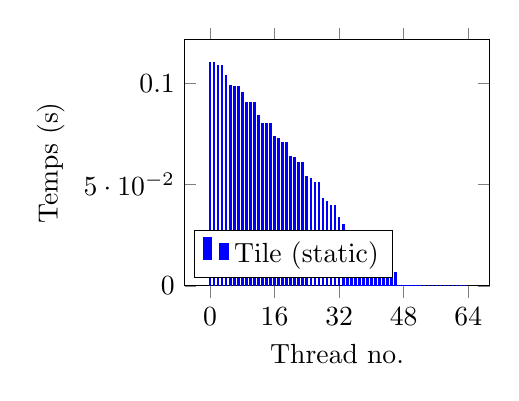
\begin{tikzpicture}
\begin{axis}[
  ybar,
  bar width=0.02cm,
  xlabel={Thread no.},
  ylabel={Temps (s)},
  ymin=0,
  legend pos=south west,
  width=0.45\textwidth,
  xtick distance=16
]

% Données pour le premier graphique (à gauche)
\addplot[color=blue, fill=blue] coordinates {
  (0,0.110371) (1,0.110372) (2,0.108850) (3,0.108710) (4,0.103807) (5,0.098983) (6,0.098203) (7,0.098199) (8,0.095442) (9,0.090408) (10,0.090374) (11,0.090645) (12,0.084239) (13,0.080211) (14,0.080087) (15,0.080165) (16,0.073587) (17,0.072880) (18,0.070579) (19,0.070547) (20,0.063993) (21,0.063152) (22,0.060868) (23,0.060832) (24,0.053840) (25,0.052891) (26,0.051035) (27,0.050983) (28,0.042897) (29,0.041709) (30,0.039737) (31,0.039668) (32,0.033445) (33,0.030411) (34,0.027182) (35,0.025835) (36,0.023326) (37,0.020621) (38,0.017917) (39,0.015985) (40,0.011304) (41,0.007567) (42,0.007572) (43,0.007569) (44,0.006975) (45,0.006990) (46,0.006743) (47,0.000197) (48,0.000190) (49,0.000188) (50,0.000190) (51,0.000190) (52,0.000184) (53,0.000182) (54,0.000183) (55,0.000182) (56,0.000188) (57,0.000188) (58,0.000187) (59,0.000189) (60,0.000197) (61,0.000197) (62,0.000196) (63,0.000197)
};
\addlegendentry{Tile (static)}

\end{axis}
\end{tikzpicture}
\hfill
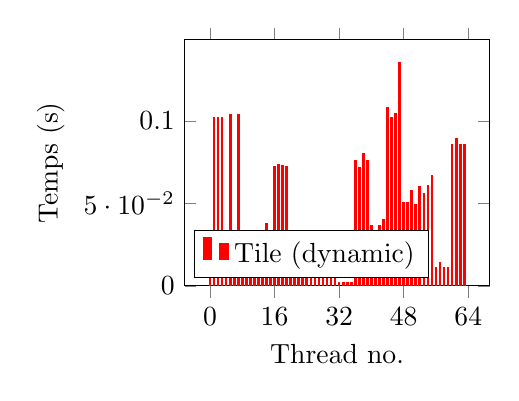
\begin{tikzpicture}
\begin{axis}[
  ybar,
  bar width=0.02cm,
  xlabel={Thread no.},
  ylabel={Temps (s)},
  ymin=0,
  legend pos=south west,
  width=0.45\textwidth,
  xtick distance=16
]

% Données pour le deuxième graphique (au milieu)
\addplot[color=red, fill=red] coordinates {
  (0,0.012374) (1,0.101916) (2,0.102231) (3,0.102335) (4,0.031646) (5,0.103791) (6,0.027345) (7,0.103736) (8,0.013294) (9,0.005048) (10,0.013196) (11,0.013274) (12,0.029977) (13,0.014822) (14,0.038031) (15,0.006773) (16,0.072430) (17,0.073348) (18,0.073030) (19,0.072646) (20,0.019042) (21,0.018557) (22,0.015584) (23,0.023265) (24,0.012978) (25,0.012921) (26,0.012991) (27,0.012913) (28,0.004344) (29,0.012693) (30,0.012060) (31,0.004269) (32,0.002005) (33,0.002045) (34,0.002016) (35,0.002037) (36,0.075942) (37,0.071761) (38,0.080139) (39,0.075963) (40,0.036564) (41,0.031572) (42,0.036697) (43,0.040236) (44,0.108409) (45,0.102279) (46,0.104325) (47,0.135749) (48,0.050331) (49,0.050334) (50,0.057982) (51,0.049150) (52,0.060416) (53,0.056260) (54,0.060576) (55,0.066686) (56,0.010841) (57,0.014129) (58,0.010829) (59,0.010865) (60,0.085464) (61,0.089510) (62,0.085493) (63,0.085527)
};
\addlegendentry{Tile (dynamic)}

\end{axis}
\end{tikzpicture}
\hfill
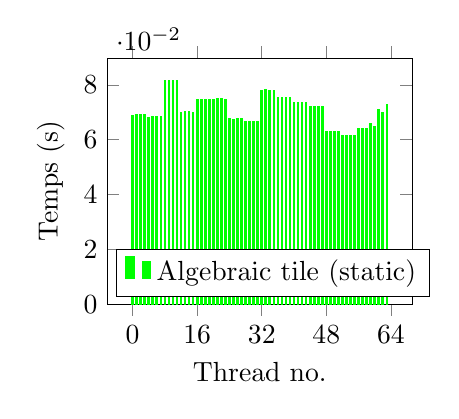
\begin{tikzpicture}
\begin{axis}[
  ybar,
  bar width=0.02cm,
  xlabel={Thread no.},
  ylabel={Temps (s)},
  ymin=0,
  legend pos=south west,
  width=0.45\textwidth,
  xtick distance=16
]

% Données pour le troisième graphique (à droite)
\addplot[color=green, fill=green] coordinates {
  (0,0.068996) (1,0.069097) (2,0.069244) (3,0.069334) (4,0.068105) (5,0.068346) (6,0.068421) (7,0.068370) (8,0.081483) (9,0.081473) (10,0.081542) (11,0.081609) (12,0.070054) (13,0.070129) (14,0.070330) (15,0.069883) (16,0.074719) (17,0.074779) (18,0.074730) (19,0.074729) (20,0.074799) (21,0.074897) (22,0.074850) (23,0.074813) (24,0.067570) (25,0.067494) (26,0.067612) (27,0.067616) (28,0.066626) (29,0.066763) (30,0.066581) (31,0.066515) (32,0.078040) (33,0.078124) (34,0.078092) (35,0.078065) (36,0.075281) (37,0.075296) (38,0.075296) (39,0.075282) (40,0.073584) (41,0.073556) (42,0.073585) (43,0.073597) (44,0.072154) (45,0.072164) (46,0.072211) (47,0.072127) (48,0.062882) (49,0.062993) (50,0.062882) (51,0.062883) (52,0.061349) (53,0.061361) (54,0.061485) (55,0.061399) (56,0.064116) (57,0.064196) (58,0.064180) (59,0.065788) (60,0.064886) (61,0.071078) (62,0.070006) (63,0.072876)
};
\addlegendentry{Algebraic tile (static)}

\end{axis}
\end{tikzpicture}

\caption{Temps d'exécution des threads pour le fichier covariance.c}
\label{fig:graphes}
\end{figure}

\begin{table}[htbp]
  \centering
  \caption{Statistiques pour le fichier covariance.c}
  \begin{tabular}{|c|c|c|c|}
    \hline
    Statistique & Algebraic Tile & Tile (static) & Tile (dynamic) \\ 
    \hline
    Skewness (g1)  & 0.121596 & 0.360362 & 0.503641 \\ 
    Kurtosis (g2)  & -0.705696 & -1.33923 & -1.01769 \\ 
    Coefficient de variation $ \frac{\sigma}{\overline{x}} $ & 0.0764234 & 0.911634 & 0.793589\\ 
    Percent Imbalance metric en \% & 15.4932 & 162.504 & 197.024\\ 
    Coefficient de Gini  & 0.0435428 & 0.513567 & 0.444867\\ 
    Temps d'exécution (s) &  0.086458 &  0.115095   &  0.150891   \\ 

    \hline
  \end{tabular}
\end{table}
g1=$ \frac{\sum_{i=1}^{n} (x_i - \overline{x})^3}{n\sigma^3} $\
g2=$ \frac{\sum_{i=1}^{n} (x_i - \overline{x})^4}{n\sigma^4} $\
Coefficient de Gini = $ \frac{\sum_{i=1}^{n}\sum_{j=1}^{n} |x_i - x_j|}{2n^2\overline{x}} $\
\newpage

  \end{document}
